\documentclass[ngerman,a4paper,order=firstname]{../../texmf/tex/latex/mathscript/mathscript}
\usepackage{../../texmf/tex/latex/mathoperators/mathoperators}

\title{\textbf{Lineare Algebra SS2018}}
\author{Dozent: Prof. Dr. Arno Fehm}

\begin{document}
\pagenumbering{roman}
\pagestyle{plain}

\maketitle

\hypertarget{tocpage}{}
\tableofcontents
\bookmark[dest=tocpage,level=1]{Inhaltsverzeichnis}

\pagebreak
\pagenumbering{arabic}
\pagestyle{fancy}

\setcounter{chapter}{4}

\chapter{Endomorphismen}
\section{Eigenwerte}

\begin{definition}[Eigenwert, Eigenvektor, Eigenraum]
	Sind $0\neq x\in V$ und $\lambda\in K$ mit $f(x)=\lambda x$ so nennt man $\lambda$ einen \begriff{Eigenwert} von $f$ und $x$ einen \begriff{Eigenvektor} von $f$ zum Eigenwert $\lambda$. Der \begriff{Eigenraum} zu $\lambda\in K$ ist $\Eig (f,\lambda)=\{x\in V\mid f(x)=\lambda x\}$.
\end{definition}

\begin{definition}[EW und EV für Matrizen]
	Sei $A\in\Mat_n(K)$. Man definiert Eigenwerte, Eigenvektoren, etc von $A$ als Eigenwerte, Eigenvektoren von $f_A\in\End_K(K^n)$.
\end{definition}
\section{Das charakteristische Polynom}

\begin{proposition}
	\proplbl{satz_det_null}
	Sei $\lambda\in K$. Genau dann ist $\lambda$ ein Eigenwert von $f$, wenn $\det(\lambda\cdot\id_V-f)=0$.
\end{proposition}
\begin{proof}
	Da $\Eig(f,\lambda)=\Ker(\lambda\cdot\id_V-f)$ ist $\lambda$ genau dann ein Eigenwert von $f$, wenn $\dim_K(\Ker(\lambda\cdot\id_V-f))>0$, also wenn $\lambda\cdot\id_V-f\notin\Aut_K(V)$. Nach \propref{4_4_6} bedeutet dies, dass $\det(\lambda\cdot\id_V-f)=0$
\end{proof}

\begin{definition}[charakteristisches Polynom]
	Das \begriff{charakteristische Polynom} einer Matrix $A\in\Mat_n(K)$ ist die Determinante der Matrix $t\cdot \mathbbm{1}_n-A\in\Mat_n(K[t])$. 
	\begin{align}
		\chi_A(t)&=\det(t\cdot \mathbbm{1}_n-A)\in K[t] \notag
	\end{align}
	Das charakteristische Polynom eines Endomorphismus $f\in\End_K(V)$ ist $\chi_f(t)=\chi_{M_B(f)}(t)$, wobei $B$ eine Basis von $V$ ist.
\end{definition}

\begin{mathematica}[charakteristisches Polynom]
	Die folgende Funktion liefert das charakteristische Polynom einer Matrix $A$ mit der Variable $x$
	\begin{align}
		\texttt{CharacteristicPolynomial[A,x]}\notag
	\end{align}
\end{mathematica}

\begin{proposition}
	\proplbl{satz_2_3}
	Sind $A,B\in\Mat_n(K)$ mit $A\sim B$, so ist $\chi_A=\chi_B$. Insbesondere ist $\chi_f$ wohldefiniert.
\end{proposition}
\begin{proof}
	Ist $B=SAS^{-1}$ mit $S\in\GL_n(K)$, so ist $t\cdot \mathbbm{1}_n-B = S(t\cdot \mathbbm{1}_n-A)S^{-1}$, also $t\cdot \mathbbm{1}_n-B\sim t\cdot \mathbbm{1}_n-A$ und ähnliche Matrizen haben die selben Determinante \propref{4_4_4}. \\
	Sind $B,B'$ Basen von $V$, so sind $M_B(f)\sim M_{B'}(f)$, also $\chi_{M_B(f)}=\chi_{M_{B'}(f)}$
\end{proof}

\begin{lemma}
	\proplbl{lemma_chi_det}
	Für $\lambda\in K$ ist $\chi_f(\lambda)=\det(\lambda\cdot\id_V-f)$.
\end{lemma}
\begin{proof}
	Sei $B$ eine Basis von $V$ und $A=M_B(f)=(a_{ij})_{i,j}$. Dann ist $M_B(\lambda\cdot\id_V-f)= \lambda\cdot \mathbbm{1}_n-A$. Aus IV.2.8 und I.6.8 folgt $\det(t\cdot \mathbbm{1}_n-A)(\lambda)=\det(\lambda\cdot \mathbbm{1}_n-A)$. Folglich ist 
	\begin{align}
		\chi_f(\lambda)&=\chi_A(\lambda)\notag \\
		&=\det(t\cdot \mathbbm{1}_n-A)(\lambda)\notag \\
		&=\det(\lambda\cdot \mathbbm{1}_n-A)\notag \\
		&= \det(\lambda\cdot\id_V-f) \notag
	\end{align}
\end{proof}

\begin{proposition}
	\proplbl{satz_chi_polynom}
	Sei $\dim_K(V)=n$ und $f\in\End_K(V)$. Dann ist $\chi_f(t)=\sum_{i=0}^n \alpha_i t^i$ ein Polynom vom Grad $n$ mit 
	\begin{align}
		\alpha_n&=1\notag \\
		\alpha_{n-1}&=-\tr(f) \notag \\
		\alpha_0 &= (-1)^n\cdot\det(f) \notag
	\end{align}
	Die Nullstellen von $\chi_f$ sind genau die Eigenwerte von $f$.
\end{proposition}
\begin{proof}
	Sei $B$ eine Basis von $V$ und $A=M_B(f)=(a_{ij})_{i,j}$. Wir erinnern uns daran, dass $\tr(f)=\tr(A=\sum_{i=1}^n a_{ii}$. Es ist $\chi_f(t)=\det(t-\cdot 1_n-A)=\sum_{\sigma\in S_n}\sgn(\sigma)\prod_{i=1}^n (t\delta_{i,\sigma(i)}-a_{i,\sigma(i)})$. \\
	Der Summand für \emph{$\sigma=\id$} ist $\prod_{i=1}^n (t-a_{ii})=t^n+\sum_{i=1}^n (-a_{ii})t^{n-1}+...+\prod_{i=1}^n(-a_{ii})$ \\
	Für \emph{$\sigma\neq\id$} ist $\sigma(i)\neq i$ für mindestens zwei $i$, der entsprechende Summand hat also Grad höchstens $n-2$. Somit haben $\alpha_n$ und $\alpha_{n-1}$ die oben behauptete Form, und $\alpha_0=\chi_A(0)=\det(-A)=(-1)^n\cdot\det(f)$. \\
	Die Aussage über die Nullstellen von $\chi_f$ folgt aus \propref{satz_det_null} und \propref{lemma_chi_det}.
\end{proof}

\begin{conclusion}
	Ist $\dim_K(V)=n$, so hat $f$ höchstens $n$ Eigenwerte.
\end{conclusion}
\begin{proof}
	\propref{satz_chi_polynom} und \propref{1_6_10}
\end{proof}

\begin{definition}[normiertes Polynom]
	Ein Polynom $0\neq P\in K[t]$ mit Leitkoeffizient 1 heißt \begriff{normiert}.
\end{definition}

\begin{example}
	\proplbl{beispiel_2_8}
	\begin{enumerate}
		\item Ist $A=(a_{ij})_{i,j}$ eine obere Dreiecksmatrix, so ist $\chi_A(t)=\prod_{i=1}^n (t-a_{ii})$, vgl. \propref{4_2_9} \\
		Insbesondere ist $\chi_{1_n}(t)=(t-1)^n$, $\chi_0(t)=t^n$
		\item Für eine Blockmatrix $A=\begin{henrysmatrix}A_1&B \\ 0&A_2\end{henrysmatrix}$ mit quadratischen Matrizen $A_1,A_2$ ist $\chi_A=\chi_{A_1}\cdot \chi_{A_2}$ vgl. \propref{4_2_9}
		\item Für
		\begin{align}
			\begin{pmatrix}
			0&...&...&...&0&-c_0  \\ 
			1& \ddots&\;&\;&\vdots&\vdots  \\ 
			0&\ddots&\ddots&\;&\vdots&\vdots  \\ 
			\vdots&\ddots&\ddots&\ddots&\vdots&\vdots  \\ 
			0&...&0&1&0&-c_{n-1} 
			\end{pmatrix} \quad c_0,...,c_{n-1}\in K \notag
		\end{align}
		ist $\chi_A(t)=t^n+\sum_{i=0}^{n-1} c_i t^i$ \\
		Man nennt diese Matrix die Begleitmatrix zum normierten Polynom $P=t^n+\sum_{i=0}^{n-1} c_i t^i$ und schreibt $M_P:=A$
	\end{enumerate}
\end{example}
\section{Diagonalisierbarkeit}

\begin{definition}[diagonalisierbar]
	Man nennt $f$ \begriff{diagonalisierbar}, wenn $V$ eine Basis $B$ besitzt, für die $M_B(f)$ eine Diagonalmatrix ist.
\end{definition}

\begin{lemma}
	\proplbl{lemma_diag_summe_eig}
	Genau dann ist $f$ diagonalisierbar, wenn
	\begin{align}
		V=\sum\limits_{\lambda\in K} \Eig(f,\lambda) \notag
	\end{align}.
\end{lemma}
\begin{proof}
	$(\Rightarrow)$: Ist $B$ eine Basis aus EV von $f$ (vgl. \propref{satz_diagonal_ev}), so ist $B\le \bigcup\limits_{\lambda\in K}\Eig(f,\lambda)$, also $V=\Span_K(\bigcup\limits_{\lambda\in K}\Eig(f, \lambda))=\sum\limits_{\lambda\in K}\Eig(f,\lambda)$. \\
	$(\Leftarrow)$: Ist $V=\sum\limits_{\lambda\in K}\Eig(f,\lambda)$, so gibt es $\lambda_1,...,\lambda_n \in K$ mit $V=\sum\limits_{i=1}^r \Eig(f,\lambda_i)$. Wir wählen Basen $B_i$ von $\Eig(f,\lambda_i)$. Dann ist $\bigcup\limits_{i=1}^r B_i$ ein endliches Erzeugendensystem von $V$, enthält also eine Basis von $V$ (II.3.6). Diese besteht aus EV von $f$. %TODO: Verlinkung
\end{proof}

\begin{proposition}
	Ist $\dim_K(V)=n$, so hat $f$ höchstens $n$ Eigenwerte. Hat $f$ genau $n$ Eigenwerte, so ist $f$ diagonalisierbar.
\end{proposition}
\begin{proof}
	Ist $\lambda$ ein EW von $f$, so ist $\dim_K(\Eig(f,\lambda))\ge 1$. Sind also $\lambda_1,...,\lambda_n$ paarweise verschiedene EW von $f$, so ist
	\begin{align}
		n=\dim_K(V)&\ge \dim_K\left( \sum\limits_{i=1}^m \Eig(f,\lambda_i)\right) \notag \\
		&\overset{\propref{satz_eig_direkte_summe}}{=} \dim_K\left( \bigoplus_{i=0}^{m} \Eig(f,\lambda_i)\right) \notag \\
		&= \sum\limits_{i=1}^m \dim_K(\Eig(f,\lambda_i)) \notag \\
		&\ge m \notag
	\end{align}
	Ist zudem $m=n$, so muss 
	\begin{align}
		\dim_K(V) &= \dim_K(\sum\limits_{i=1}^m \Eig(f,\lambda_i))\text{ sein, also }\notag \\
		V&= \sum\limits_{i=1}^m \Eig(f,\lambda_i) \notag
	\end{align}
	Nach \propref{lemma_diag_summe_eig} ist $f$ genau dann diagonalisierbar.
\end{proof}

\begin{definition}[$a$ teilt $b$]
	Sei $R$ ein kommutativer Ring mit seien $a,b\in R$. Man sagt, $a$ \begriff{teilt} $b$ (in Zeichen $a\vert b$), wenn es $x\in R$ mit $b=ax$ gibt.
\end{definition}

\begin{definition}[Vielfachheit]
	Für $0\neq P\in K[t]$ und $\lambda\in K$ nennt man $\mu(P,\lambda)=\max\{r\in \natur_{>0}\mid (t-r)^r\vert P\}$ die \begriff{Vielfachheit} der Nullstelle $\lambda$ von $P$.
\end{definition}

\begin{lemma}
	Genau dann ist $\mu(P,\lambda)\ge 1$, wenn $\lambda$ eine Nullstelle von $P$ ist.
\end{lemma}
\begin{proof}
	$(\Rightarrow)$: $t-\lambda\vert P\Rightarrow P(t)=(t-\lambda)\cdot Q(t)$ mit $Q(t)\in K[t]\Rightarrow P(\lambda)=0\cdot Q(\lambda)=0$. \\
	$(\Leftarrow)$: $P(\lambda)=0\overset{I.6.9}{=}t-\lambda\vert P(t)\Rightarrow \mu(P,\lambda)\ge 1$.
	%TODO: Verlinkung
\end{proof}

\begin{lemma}
	Ist $P(t)=(t-\lambda)^r\cdot Q(t)$ mit $Q(t)\in K[t]$ und $Q(\lambda)\neq 0$, so ist $\mu(P,\lambda)=r$
\end{lemma}
\begin{proof}
	Offensichtlich ist $\mu(P,\lambda)\ge r$. Wäre $\mu(P,\lambda)\ge r+l$, so $(t-\lambda)^{r+l}\vert P(t)$ also $(t-\lambda)^r\cdot Q(t)=(t-\lambda)^{r^+l}\cdot R(t)$ mit $R(t)\in K[t]$, folglich $t-\lambda\vert Q(t)$, insbesondere $Q(\lambda)=0$. \\
	(Denn wir dürfen kürzen: $R$ ist Nullteilerfrei, genau so wie $K[t]$). \\
	$(t-\lambda)^r(Q(t)-(t-\lambda)R(t))=0\Rightarrow Q(t)=(t-\lambda)R(t)$.
\end{proof}
\section{Trigonalisierbarkeit}

\begin{definition}
	Man nennt $f$ \begriff{trigonalisierbar}, wenn $V$ eine Basis $B$ besitzt, für die $M_B(f)$ eine obere Dreiecksmatrix ist.
\end{definition}

\begin{definition}[invariant]
	Ein Untervektorraum $W\le V$ ist $f$-\begriff{invariant}, wenn $f(W)\le W$.
\end{definition}
\section{Das Minimalpolynom}

\begin{definition}
	Für ein Polynom $P(t)=\sum_{i=0}^n c_it^i\in K[t]$ definieren wir $P(f)=\sum_{i=0}^m c_if^i\in\End_K(V)$, wobei $f^0=\id_V$, $f^1=f$, $f^2=f\circ f$, ...
	
	Analog definiert man $P(A)$ für $A\in\Mat_n(K)$.
\end{definition}

\begin{remark}
	\proplbl{5_5_2}
	Die Abbildung
	\begin{align}
		\begin{cases}
			K[t]\to \End_K(V)\\ P\mapsto P(f)
		\end{cases}\notag
	\end{align}
	ist ein Homomorphismus von $K$-Vektorraum und Ringen. Sein Kern ist das Ideal 
	\begin{align}
		\mathcal{I}_f:=\{P\in K[t]\mid P(f)=0\}\notag
	\end{align}
	und sein Bild ist der kommutative Unterring 
	\begin{align}
		K[f]:&=\{P(f)\mid P\in K[t]\}\notag \\
		&= \Span_K(f^0,f^1,f^2,...)\notag
	\end{align}
	des (im Allgemeinen nicht kommutativen) Rings $\End_K(V)$.
	
	Analog definiert man $\mathcal{I}_A$ und $K[A]\le \Mat_n(K)$.
\end{remark}

\begin{lemma}
	\proplbl{lemma_5_3}
	$\mathcal{I}_f\neq\{0\}$
\end{lemma}
\begin{proof}
	Wäre $\mathcal{I}_f=\{0\}$, so wäre $K[t]\to \End_K(V)$ injektiv, aber $\dim_K(K[t])= \infty>n^2=\dim_K(\End_K(V))$, ein Widerspruch.
\end{proof}

\begin{proposition}
	\proplbl{satz_5_4}
	Es gibt ein eindeutig bestimmtes normiertes Polynom $0\neq P\in K[t]$ kleinsten Grades mit $P(f)=0$. Dieses teilt jedes $Q\in K[t]$ mit $Q(f)=0$.
\end{proposition}
\begin{proof}
	Nach \propref{lemma_5_3} gibt es $0\neq P\in K[t]$ mit $P(f)=0$ von minimalem Grad $d$. Indem wir durch den Leitkoeffizienten von $P$ teilen, können wir annehmen, dass $P$ normiert ist. \\
	Sei $Q\in\mathcal{I}_f$. Polynomdivision liefert $R,H\in K[t]$ mit $Q=P\cdot H+R$ und $\deg(R)<\deg(P)=d$. Es folgt $R(f)=\underbrace{Q(f)}_{=0}-\underbrace{P(f)}_{=0}\cdot H(f)=0$. Aus der Minimalität von $d$ folgt $R=0$ und somit $P\mid Q$. \\
	Ist $Q$ zudem normiert vom Grad $d$, so ist $H=1$, also $Q=P$, was die Eindeutigkeit zeigt.
\end{proof}

\begin{definition}[Minimalpolynom]
	Das eindeutig bestimmte normierte Polynom $0\neq P\in K[t]$ kleinsten Grades mit $P(f)=0$ nennt man das \begriff{Minimalpolynom} $P_f$ von $f$.
	
	Analog definiert man das Minimalpolynom $P_A\in K[t]$ einer Matrix $A\in\Mat_n(K)$.
\end{definition}

\begin{mathematica}[Minimalpolynom]
	Die Funktion für das Minimalpolynom $p$ mit der Variable $t$ von einer Matrix $A$ in Mathematica bzw. WolframAlpha lautet:
	\begin{align}
		\texttt{MinimalPolynomial[A,x]}\notag
	\end{align}
\end{mathematica}

\begin{example}
	\begin{enumerate}
		\item $A=\mathbbm{1}_n$, $\chi_A(t)=(t-1)^n$, $P_A(t)=t-1$
		\item $A=0$, $\chi_A(t)=t^n$, $P_A(t)=t$
		\item Ist $A=\diag(a_1,...,a_n)$ mit paarweise verschiedenen Eigenwerten $\lambda_1,...,\lambda_r$, so ist $\chi_A(t)=\prod_{i=1}^n (t-a_i)=\prod_{i=1}^n (t-\lambda_i)^{\mu_a(f_A,\lambda_i)}$, $P_A(t)=\prod_{i=1}^r (t-\lambda_i)$ und es folgt $\deg(P_A)\ge \vert \{a_1,...,a_n\}\vert=r$.
	\end{enumerate}
\end{example}

\begin{definition}[$f$-zyklisch]
	Ein $f$-invarianter Untervektorraum $W\le V$ heißt $f$-\begriff{zyklisch}, wenn es ein $x\in W$ mit $W=\Span_K(x,f(x),f^2(x),...)$ gibt.
\end{definition}

\begin{lemma}
	\proplbl{lemma_5_8}
	Sei $x\in V$ und $x_i=f^i(x)$. Es gibt ein kleinstes $k$ mit $x_k\in\Span_K(x_0,x_1,...,x_{k-1})$, und $W=\Span_K(x_0,...,x_{k-1})$ ein $f$-zyklischer Untervektorraum von $V$ mit Basis $B=(x_0,...,x_{k-1})$ und $M_B(f\vert_W)=M_{\chi_{f\vert_W}}$.
\end{lemma}
\begin{proof}
	Da $\dim_K(V)=n$ ist $(x_0,...,x_n)$ linear abhängig, es gibt also ein kleinstes $k$ mit $(x_0,...,x_{k-1})$ linear unabhängig, aber $(x_0,...,x_k)$ linear abhängig, folglich $x_k\in\Span_K(x_0,...,x_{k-1})$. Mit $x_k=f(x_{k-1})=\sum_{i=0}^{k-1}-c_ix_i$ ist dann 
	Da $\dim_K(V)=n$ ist $(x_0,...,x_n)$ linear abhängig, es gibt also ein kleinstes $k$ mit $(x_0,...,x_{k-1})$ linear unabhängig, aber $(x_0,...,x_k)$ linear abhängig, folglich $x_k\in\Span_K(x_0,...,x_{k-1})$. Mit $x_k=f(x_{k-1})=\sum_{i=0}^{k-1}-c_ix_i$ ist dann 
	\begin{align}
		M_B(f\vert_W)=\begin{pmatrix}0&...&...&...&0&-c_0\\
		1&\ddots&\;&\;&\vdots&\vdots\\
		0&\ddots&\ddots&\;&\vdots&\vdots\\
		\vdots&\ddots&\ddots&\ddots&\vdots&\vdots\\
		0&...&0&1&0&-c_{k-1}\end{pmatrix}\notag
	\end{align}
	somit $\chi_{f\vert_W}=t^k+\sum_{i=0}^{k-1}c_it^i$, also $M_B(f\vert_W)=M_{\chi_{f\vert_W}}$.
\end{proof}

\begin{theorem}[Satz von \person{Cayley-Hamilton}]
	\proplbl{theorem_5_9}
	Für $f\in\End_K(V)$ ist $\chi_f(f)=0$.
\end{theorem}
\begin{proof}
	Sei $x\in V$. Definiere $x_i=f^i(x)$ und $W=\Span_K(x_0,...,x_{k-1})$ wie in \propref{lemma_5_8}. Sei $\chi_{f\vert_W}=t^k+\sum_{i=0}^{k-1} c_it^i$, also $f(x_{k-1})=\sum_{i=0}^{k-1} -c_ix_i$. Wenden wir $\chi_{f\vert_W}(f)\in\End_K(V)$ auf $x$ an, so erhalten wir 
	\begin{align}
		\chi_{f\vert_W}(f)(x)&=\left( f^k+\sum\limits_{i=1}^{k-1} c_if^i\right)(x)\notag \\
		&= \sum\limits_{i=1}^{k-1} -c_ix_i+\sum\limits_{i=1}^{k-1}c_ix_i\notag \\
		&= 0\notag
	\end{align}
	Aus $\chi_{f\vert_W}\mid \chi_f$ (\propref{beispiel_4_6}) folgt somit $\chi_f(f)(x)=0$, denn ist $\chi_f=Q\cdot \chi_{f\vert_W}$ mit $Q\in K[t]$, so ist $\chi_f(f)=Q(f)\circ\chi_{f\vert_W}(f)$, also $\chi_f(f)(x)=Q(f)(\underbrace{\chi_{f\vert_W}(f)(x)}_{=0})=0$. Da $x\in V$ beliebig war, folgt $\chi_f(f)=0\in\End_K(V)$.
\end{proof}

\begin{conclusion}
	\proplbl{folgerung_5_10}
	Es gilt $P_f\mid \chi_f$. Insbesondere ist $\deg(P_f)\le n$.
\end{conclusion}
\begin{proof}
	\propref{theorem_5_9} + \propref{satz_5_4}
\end{proof}

\begin{remark}
	Ist $B$ eine Basis von $V$ und $A=M_B(f)$, so ist $P_A=P_f$. Insbesondere ist $P_A=P_B$ für $A\sim B$. Als Spezialfall von \propref{theorem_5_9} erhält man $\chi_A(A)=0$ und $P_A\mid \chi_A$.
\end{remark}

\begin{remark}
	Der naheliegende "'Beweis"' $\underbrace{\chi_A}_{\in\Mat_n(K)}=\det(t\mathbbm{1}_n-A)(A) =\det(A\mathbbm{1}_n-A)=\det(0)=\underbrace{0}_{\in K}$ ist falsch!
\end{remark}

\section{Nilpotente Endomorphismen}

\begin{remark}
	Für $f\in\End_K(V)$ sind 
	\begin{itemize}
		\item $f\{0\}=\Ker(f^0)\subseteq \Ker(f^1)\subseteq \Ker(f^2)\subseteq ...$
		\item $V=\Image(f^0)\supseteq \Image(f^1)\supseteq \Image(f^2)\supseteq ...$
	\end{itemize}
Folgen von UVR von $V$. Nach der Kern-Bild-Formel III.7.13 ist %TODO: Verlinkung
\begin{align}
	\dim_K(\Ker(f^i))+\dim_K(\Image(f^i))=\dim_K(V)\quad\forall i\notag
\end{align}
Da $\dim_K(V)=n<\infty$ gibt es ein $d$ mit $\Ker(f^d)=\Ker(f^{d+i})$ und $\Image(f^d)=\Image(f^{d+i})$ für jedes $i\ge 0$.
\end{remark}

\begin{example}
	$f=f_A$, $A\in\Mat_2(K)$.
	\begin{itemize}
		\item $A=\begin{pmatrix}1&0\\0&1\end{pmatrix}$: $\{0\}=\Ker(f^0)=\Ker(f^1)=...$
		\item $A=\begin{pmatrix}1&0\\0&0\end{pmatrix}$: $\{0\}=\Ker(f^0)\subset\Ker(f^1)=\Ker(f^2)=...=\Span_K(e_2)$
		\item $A=\begin{pmatrix}0&1\\0&0\end{pmatrix}$: $\{0\}=\Ker(f^0)\subset\underbrace{\Ker(f^1)}_{=\Span_K(e_1)}\subset \Ker(f^2)=... = K^2$
		\item $A=\begin{pmatrix}0&0\\0&0\end{pmatrix}$: $\{0\}=\Ker(f^0)\subset\Ker(f^1)=\Ker(f^2)=...=K^2$
	\end{itemize}
\end{example}

\begin{lemma}
	\proplbl{lemma_6_3}
	Seien $f,g\in\End_K(V)$. Wenn $f$ und  $g$ kommutieren, d.h. $f\circ g=g\circ f$, so sind die UVR $\Ker(g)$ und $\Image(g)$ $f$ invariant.
\end{lemma}
\begin{proof}
	Ist $x\in\Ker(f)$, so ist $g(f(x))=f(g(x))=f(0)=0$, also $f(x)\in\Ker(g)$. Für $g(x)\in\Image(g)$ ist $f(g(x))=g(f(x))\in\Image(g)$.
\end{proof}

\begin{proposition}[Lemma von \person{Fitting}]
	Seien $V_i=\Ker(f^i)$, $W_i=\Image(f^i)$, $d=\min\{i:V_i=V_{i+1}\}$. Dann sind 
	\begin{align}
		\{0\}&=V_0\subset V_1\subset ...\subset V_d=V_{d+1}=...\notag \\
		V&= W_0\supset W_1\supset ... \supset W_d=W_{d+1}=...\notag
	\end{align}
	Folgen $f$-invarianter UVR und $V=V_d\oplus W_d$.
\end{proposition}
\begin{proof}
	Da $f^i$ und $f^j$ für beliebige $i,j$ kommutieren, sind $V_i$ und $V_j$ nach \propref{lemma_6_3} $f$-invariant für jedes $i$. Aus $\dim_K(V_i)+\dim_K(W_i)=n$ folgt $d=\min\{i:W_i=W_{i+1}\}$, insbesondere ist $\Image(f^d)=\Image(f^{d+1})=f(\Image(f^d))$, somit $W_{d+i}=\Image(f^{d+i})=W_d$ für $i\ge 0$, also auch $V_d=V_{d+i}$ für alle $i\ge 0$. \\
	Insbesondere ist $f^d\vert_{W_d}:W_d\to W_{2d}=W_d$ surjektiv, also auch injektiv, also $V_d\cap W_d=\{0\}$. Aus der Dimensionsformel II.4.12 folgt dann $\dim_K(V_d+W_d)=\dim_K(V_d)+\dim_K(W_d)=\dim_K(V)$. Folglich ist $V_d+W_d=V$ und $V_d\cap W_d=\{0\}$, also $V=V_d\oplus W_d$.
\end{proof}

\begin{definition}[nilpotent]
	Ein $f\in\End_K(V)$ heißt \begriff{nilpotent}, wenn $f^k=0$ für ein $k\in\natur$. Analog heißt $A\in\Mat_n(K)$ nilpotent, wenn $A^k=0$ für $k\in\natur$. Das kleinste $k$ mit $f^k=0$ bzw. $A^k$ heißt die \begriff{Nilpotenzklasse} von $f$ bzw. $A$.
\end{definition}

\begin{lemma}
	Ist $f$ nilpotent, so gibt es eine Basis $B$ von $V$, für die $M_B(f)$ eine strikte obere Dreiecksmatrix ist.
\end{lemma}
\begin{proof}
	Induktion nach $n=\dim_K(V)$. \\
	\emph{$n=1$}: $f^k=0\Rightarrow f=0$ \\
	\emph{$n>1$}: Sei $k$ die Nilpotenzklasse von $f$ und $U=\Ker(f^{k-1})$. Dann ist $U\subset V$. Da $f^k=f^{k-1}\circ f$ ist $f(V\subset U$, insbesondere $f\vert_U\in\End_K(U)$. Da $f\vert_U$ nilpotent ist, gibt es nach I.H. eine Basis $B_0$ von $U$, für die $M_B(f\vert_U)$ eine strikte obere Dreiecksmatrix ist. Ergänze $B_0$ zu einer Basis $B$ von $V$. Da $f(V)\subset U$ ist dann auch 
	\begin{align}
		M_B(f)=\begin{pmatrix}M_{B_0}(f\vert-U)&*\\0&0\end{pmatrix}\notag
	\end{align}
	eine strikte obere Dreiecksmatrix.
\end{proof}
\section{Die \person{Jordan}-Normalform}

\begin{definition}[Hauptraum]
	Der \begriff{Hauptraum} von $f$ zum Eigenwert $\lambda$ der Vielfachheit $r=\mu_a(f,\lambda)$ ist
	\begin{align}
		\Hau(f,\lambda)=\Ker\Big( (f-\lambda\id_V)^r\Big) \notag
	\end{align}
\end{definition}

\begin{lemma}
	\proplbl{lemma_7_2}
	$\Hau(f,\lambda)$ ist ein $f$-invarianter Untervektorraum der Dimension $\dim_K(\Hau(f,\lambda))= \mu_a(f,\lambda)$, auf dem $f-\lambda\id_V$ nilpotent ist und $\chi_{f\vert_{\Hau(f,\lambda)}}= (t-\lambda)^{\mu_a(f,\lambda)}$
\end{lemma}
\begin{proof}
	$f$ kommutiert sowohl mit $f$ als auch mit $\id_V$, somit auch mit $(f-\lambda\id_V)^r$. Die $f$-Invarianz von $U=\Hau(f,\lambda)$ folgt aus \propref{lemma_6_3}. Nach \propref{folgerung_6_9} ist $\dim_K(U)=\mu_a(f-\lambda\id_V,0)$ und da $\chi_f(t)=\chi_{f-\lambda\id_V}(t-\lambda)$ ist $\mu_a(f,\lambda)=\mu(\chi_f,\lambda)= \mu_a(f-\lambda\id_V,0)$. Da $f-\lambda\id_V\vert_U$ nilpotent ist $\chi_{f-\lambda\id_V\vert_U}(t)= t^r$, somit $\chi_{f\vert_U}(t)=(t-\lambda)^r$.
\end{proof}

\begin{proposition}[Hauptraumzerlegung]
	\proplbl{satz_7_3}
	Ist $\chi_f(t)=\prod_{i=1}^m (t-\lambda_i)^{r_i}$ mit $\lambda_1,...,\lambda_m\in K$ paarweise verschieden und $r_1,...,r_m\in\natur$, so ist $V=\bigoplus_{i=1}^m V_i$ mit $V_i=\Hau(f,\lambda_i)$ eine Zerlegung in $f$-invariante Untervektorräume und für jedes $i$ ist $\chi_{f\vert_{V_i}}(t)=(t-\lambda_i)^{r_i}$.
\end{proposition}
\begin{proof}
	Induktion nach $m$.\\
	\emph{$m=1$}: $r_1=n\overset{\propref{lemma_7_2}}{\Rightarrow} V=V_1$.\\
	\emph{$m-1\to m$}: Nach \propref{satz_6_4} ist $V=V_1\oplus W_1$ mit $W_1=\Image((f-\lambda_i\id_V)^r)$ eine Zerlegung in $f$-invariante Untervektorräume mit $\dim_K(V_1)=r_1$, $\dim_K(W_1)=n-r_1$. Somit ist $\chi_f=\chi_{f\vert_{V_1}}\cdot \chi_{f\vert_{W_1}}$ und $\chi_{f\vert_{V_1}}\overset{\propref{lemma_7_2}}{=}(t-\lambda_1)^{r_1}$ also $\chi_{f\vert_{W_1}}=\prod_{i=2}^m (t-\lambda_i)^{r_i}$. Nach I.H. ist also $W_1=\bigoplus_{i=2}^m \Hau(f\vert_{W_1},\lambda_i)$. Es ist für $i\ge 2$ $\Hau(f\vert_{W_1},\lambda_i)\subseteq\Hau(f,\lambda_i)=V_i$ und da $\dim_K(\Hau(f\vert_{W_1},\lambda_i))=r_i=\dim_K(\Hau(f,\lambda_i))$ gilt Gleichheit. Damit ist
	\begin{align}
		V&=V_1\oplus W_1 \notag\\
		&=V_1\oplus\bigoplus_{i=2}^m\Hau(f\vert_{W_1},\lambda_i)\notag \\
		&= V_1\oplus\bigoplus_{i=2}^m V_i \notag\\
		&= \bigoplus_{i=1}^m V_i\notag
	\end{align}
\end{proof}

\begin{example}
	$f=f_A$
	\begin{align}
		A=\begin{pmatrix}1&3&\; \\ \;&1&4 \\ \;&\; & 2\end{pmatrix}\in\Mat_3(\real)\notag
	\end{align}
	$\chi_A(t)=(t-1)^2(t-2)$
	$\Rightarrow \real^3=\underbrace{\Hau(f,1)}_{\dim = 2}\oplus\underbrace{\Hau(f,2)}_{\dim = 1}$ \\
	$\Hau(f,1)=\Ker((f-\id)^2)=L((A-\mathbbm{1})^2,0)$ \\
	$\Hau(f,2)=\Ker(f-2\id)=\Eig(f,2)=L(A-2\mathbbm{1},0)$ \\
	\begin{align}
		A-\mathbbm{1}&=\begin{henrysmatrix}0&3&\; \\ \; & -1&4 \\ \;&\;&0\end{henrysmatrix}, (A-\mathbbm{1})^2=\begin{henrysmatrix}0&\;&12 \\ \;&0&4 \\ \;&\;&1\end{henrysmatrix}&\Rightarrow \Hau(f,1)=\real e_1+\real e_2\notag \\
		A-2\mathbbm{1}&=\begin{henrysmatrix}-1&3&\; \\ \; & -1&4 \\ \;&\;&0\end{henrysmatrix}&\Rightarrow\Hau(f,2)=\real\begin{henrysmatrix}12\\4\\1\end{henrysmatrix}\notag
	\end{align}
	Mit $B=\left( \begin{henrysmatrix}1\\0\\0\end{henrysmatrix}, \begin{henrysmatrix}0\\1\\0\end{henrysmatrix}, \begin{henrysmatrix}12\\4\\1\end{henrysmatrix}\right) $ ist
	\begin{align}
		M_B(f)=\begin{pmatrix}\begin{pmatrix}1&3\\\; & 1\end{pmatrix}&\; \\ \; & 2\end{pmatrix}\notag
	\end{align} 
\end{example}

\begin{theorem}[\person{Jordan}-Normalform]
	Sei $f\in\End_K(V)$ ein Endomorphismus, dessen charakteristisches Polynom $\chi_f$ in Linearfaktoren zerfällt. Dann gibt es $r\in\natur$, $\mu_1,...,\mu_r\in K$ und $k_1,...,k_r\in \natur$ mit $\sum_{i=1}^r k_i=\dim_K(V)$ und eine Basis $B$ von $V$ mit
	\begin{align}
		M_B(f)=\diag(J_{k_1}(\mu_1),...,J_{k_r}(\mu_r))\notag
	\end{align} 
	Die Paare $(\mu_1,k_1),...,(\mu_r,k_r)$ heißen die \begriff{\person{Jordan}-Invarianten} von $f$ und sind bis auf Reihenfolge eindeutig bestimmt.
\end{theorem}
\begin{proof}
	Schreibe $\chi_f(t)=\prod_{i=1}^m (t-\lambda_i)^{r_i}$ mit $\lambda_1,...,\lambda_m\in K$ paarweise verschieden, $r_i\in\natur$. Sei $V_i=\Hau(f,\lambda_i)$. Nach \propref{satz_7_3} ist $V=\bigoplus_{i=1}^m V_i$ eine Zerlegung in $f$-invariante Untervektorräume. Für jedes $i$ wenden wir \propref{satz_6_13} auf $(f-\lambda_i\id_V)\vert_{V_i}$ an und erhalten eine Basis $B_i$ von $V_i$ und $k_{i,1}\ge ...\ge k_{i,s_i}$ mit 
	\begin{align}
		M_B((f-\lambda_i\id)\vert_{V_i})=\diag(J_{k_{i,1}},...,J_{k_{i,s_i}})\notag
	\end{align}
	Es folgt $M_{B_i}(f\vert_{V_i})=M_{B_i}(\lambda_i\id_{V_i})+M_{B_i}((f-\lambda_i\id_V)\vert_{V_i})$. Ist nun $B$ die Vereinigung der $B_i$, so hat $M_B(f)$ die gewünschte Form. Die Eindeutigkeit der \person{Jordan}-Invarianten folgt aus der Eindeutigkeit der $k_{i,j}$ in \propref{lemma_6_3}.
\end{proof}

\begin{remark}
	Ist $K$ algebraisch abgeschlossen, so haben wir nun eine (bis auf Permutationen) eindeutige Normalform für Endomorphismen $f\in\End_K(V)$ gefunden. Aus ihr lassen sich viele Eigenschaften des Endomorphismus leicht ablesen.
\end{remark}

\begin{conclusion}
	\proplbl{folgerung_7_7}
	Sei $f\in\End_K(V)$ trigonalisierbar mit $\chi_f(t)=\prod_{i=1}^m (t-\lambda_i)^{\mu_a(f,\lambda_i)}$, $P_f(t)=\prod_{i=1}^m (t-\lambda_i)^{d_i}$ und \person{Jordan}-Invarianten $(\mu_1,k_1),...,(\mu_r,k_r)$. Mit $J_i=\{j\mid \mu_j=\lambda_i\}$ ist dann 
	\begin{align}
		\mu_g(f,\lambda_i)&= \vert J_i \vert \notag \\
		\mu_a(f,\lambda_i) &= \sum_{j\in J_i} k_j\notag \\
		d_i&= \max\{k_j\mid j\in J_i\}\notag
	\end{align}
\end{conclusion}
\begin{proof}
	\begin{itemize}
		\item $\mu_a$: klar, da $\chi_f(t)=\prod_{j=1}^r (t-\mu_j)^{k_j}=\prod_{i=1}^m (t-\lambda_i)^{\mu_a(f,\lambda_i)}$
		\item $\mu_g$: lese Basis von $\Eig(f,\lambda_i)$ aus \person{Jordan}-NF: Jeder Block $J_{k_j}(\lambda_i)$ liefert ein Element der Basis.
		\item $d_i$: folgt, da $J_{k_j}$ nilpotent von Nilpotenzklasse $k_j$ ist (\propref{lemma_6_12}).
	\end{itemize}
\end{proof}

\begin{conclusion}
	Genau dann ist $f$ diagonalisierbar, wenn 
	\begin{align}
		\chi_f(t)&=\prod_{i=1}^m (t-\lambda_i)^{r_i}\quad \lambda_1,...,\lambda_m\in K\text{ paarweise verscheiden und} \notag \\
		P_f(t) &= \prod_{i=1}^m (t-\lambda_i)\notag
	\end{align}
\end{conclusion}
\begin{proof}
	Genau dann ist $f$ diagonalisierbar, wenn $f$ trigonalisierbar ist und die \person{Jordan}-NF die Diagonalmatrix ist (Eindeutigkeit der JNF), also $k_j=1$ für alle $j$. Nach \propref{folgerung_7_7} ist dies äquivalent dazu, dass $d_i=1$ für alle $i$, also $P_f=\prod_{i=1}^m (t-\lambda_i)$.
\end{proof}

\begin{remark}
	Wieder definiert man die \person{Jordan}-Invarianten, etc. von einer Matrix $A\in\Mat_n(K)$ als die \person{Jordan}-Invarianten von $f_A\in\End_K(K^n)$.
\end{remark}

\begin{conclusion}
	Seien $A,B\in\Mat_n(K)$ trigonalisierbar. Genau dann ist $A\sim B$, wenn $A$ und $B$ die gleichen \person{Jordan}-Invarianten haben.
\end{conclusion}
\begin{proof}
	Existenz und Eindeutigkeit der \person{Jordan}-Normalform.
\end{proof}

\chapter{Skalarprodukte}
In diesem ganzen Kapitel seien
\begin{itemize}
	\item $K=\real$ oder $K=\comp$
	\item $n\in\natur$
	\item $V$ ein $n$-dimensionaler $K$-VR
\end{itemize}

\section{Das Standardskalarprodukt}

Sei zunächst $K=\real$.

\begin{definition}[Standardskalarprodukt in $\real$]
	Auf den Standardraum $V=\real^n$ definiert man das \begriff{Standardskalarprodukt in $\real$} $\langle.\rangle:\real^n\times\real^n\to \real$ durch
	\begin{align}
		\skalar{x}{y}=x^ty=\sum_{i=1}^n x_iy_i\notag
	\end{align}
\end{definition}

Sei nun $K=\comp$.

\begin{definition}[komplexe Konjugation, Absolutbetrag]
	Für $x,y\in\real$ und $z=x+iy\in\comp$ definiert man $\overline{z}=x-iy$ heißt \begriff{komplexe Konjugation}.. Man definiert den \begriff{Absolutbetrag} von $z$ als
	\begin{align}
		\vert z\vert &=\sqrt{z\overline{z}}=\sqrt{x^2+y^2}\in\real_{\ge 0}\notag
	\end{align}
	Für $A=(a_{ij})_{i,j}\in\Mat_{m\times n}(\comp)$ sehen wir
	\begin{align}
		\overline{A}&= (\overline{a_{ij}})_{i,j}\in\Mat_{m\times n}(\comp)\notag
	\end{align}
\end{definition}

\begin{definition}[Standardskalarprodukt in $\comp$]
	Auf $K=\comp^n$ definiert man das \begriff{Standardskalarprodukt in $\comp$} $\langle\cdot,\cdot\rangle:\comp^n\times\comp^n\to \comp$ durch
	\begin{align}
	\langle x,y\rangle=x^t\overline{y}=\sum_{i=1}^n x_i\overline{y}_i\notag
	\end{align}
\end{definition}

\begin{definition}[euklidische Norm in $\comp$]
	Auf $V=\comp$ definiert man die \begriff{euklidische Norm in $\comp$} $\Vert \cdot \Vert:\comp^n\to \real_{\ge 0}$ durch
	\begin{align}
	\Vert x\Vert =\sqrt{\langle  x,x\rangle}\notag
	\end{align}
\end{definition}
\section{Bilinearformen und Sesquilinearformen}

Sei $K=\real$ oder $K=\comp$.

\begin{definition}[Bilinearform, Sesquilinearform]
	Eine \begriff{Bilinearform} ($K=\real$) bzw. \begriff{Sesquilinearform} ($K=\comp$) ist eine Abbildung $s:V\times V\to K$ für die gilt:
	\begin{itemize}
		\item Für $x,x',y\in V$ ist $s(x+x',y)=s(x,y)+s(x',y)$
		\item Für $x,y,y'\in V$ ist $s(x,y+y')=s(x,y)+s(x,y')$
		\item Für $x,y\in V$, $\lambda\in K$ ist $s(\lambda x,y)=\lambda s(x,y)$
		\item Für $x,y\in V$, $\lambda\in K$ ist $s(x,\lambda y)=\kringel{white}{\overline{\lambda}} s(x,y)$
	\end{itemize}
\end{definition}

\begin{remark}
	Im Fall $K=\real$ ist $\lambda=\overline{\lambda}$. Wir werden der Einfachheit halber auch in diesem Fall von Sesquilinearformen sprechen, vgl. \propref{6_1_12}
\end{remark}

\begin{example}
	Für $A=(a_{ij})_{i,j}\in\Mat_n(K)$ ist $s_A:K^n\times K^n\to K^n$ gegeben durch
	\begin{align}
		s_A(x,y)=x^tA\overline{y}=x^t\left( \sum_{j=1}^n a_{ij}\overline{y}_j\right)_i=\sum_{i,j=1}^n a_{ij}x_i\overline{y}_j\notag
	\end{align}
	eine Sesquilinearform auf $V=K^n$.
\end{example}

\begin{definition}
	Sei $s$ eine Sesquilinearform auf $V$ und $B=(v_1,...,v_n)$ eine Basis von $V$. Die \begriff[Sesquilinearform!]{darstellende Matrix} von $s$ bzgl. $B$ ist
	\begin{align}
		M_B(s)=(s(v_i,v_j))_{i,j}\in\Mat_n(K)\notag
	\end{align}
\end{definition}

\begin{example}
	Die darstellende Matrix des Standardskalarprodukts $s=s_{\mathbbm{1}_n}$ auf den Standardraum $V=K^n$ bzgl. der Standardbasis $\mathcal{E}$ ist
	\begin{align}
		M_{\mathcal{E}}(s)=\mathbbm{1}_n\notag
	\end{align}
\end{example}

\begin{lemma}
	\proplbl{6_2_6}
	Seien $v,w\in V$. Mit $x=\Phi_B^{-1}(v)$, $y=\Phi_B^{-1}(w)$ und $A=M_B(s)$ ist $s(v,w)=x^tA\overline{y}=s_A(x,y)$.
\end{lemma}
\begin{proof}
	Achtung: $v_i$ beschreibt das $i$-te Element der Basis $B$!\\
	$s(v,w)=s(\sum_{i=1}^n x_iv_i,\sum_{j=1}^n y_jv_j)=\sum_{i,j=1}^n x_i\overline{y}s(v,v_j)=x^tA\overline{y}$
\end{proof}

\begin{proposition}
	Sei $B$ eine Basis von $V$. Die Abbildung $s\mapsto M_B(s)$ ist eine Bijektion zwischen den Sesquilinearformen auf $V$ und $\Mat_n(K)$.
\end{proposition}
\begin{proof}
	\begin{itemize}
		\item injektiv: \propref{6_2_6}
		\item surjektiv: Für $A\in\Mat_n(K)$ wird durch $s(v,w)=\Phi_B^{-1}(v)^t\cdot A\cdot \overline{\Phi_B^{-1}(w)}$ eine Sesquilinearform auf $V$ mit $M_B(s)=(s(v_i,w_j))_{i,j}= (e_i^tA\overline{e_j})_{i,j}=(e_iAe_j)_{i,j}=A$ definiert.
	\end{itemize}
\end{proof}

\begin{proposition}[Transformationsformel]
	\proplbl{6_2_8}
	Seien $B$ und $B'$ Basen von $V$ und $s$ eine Sesquilinearform auf $V$. Dann gilt:
	\begin{align}
		M_{B'}(s)=(T_B^{B'})^t\cdot M_B(s)\cdot \overline{T_B^{B'}}\notag
	\end{align}
\end{proposition}
\begin{proof}
	Seien $v,w\in V$. Definiere $A=M_B(s)$, $A'=M_{B'}(s)$, $T=T_B^{B'}$ und $x,y,x',y'\in K^n$ mit $v=\Phi_B(x)=\Phi_B(x')$, $w=\Phi_B(y)=\Phi_B(y')$. Dann ist $x=Tx'$, $y=Ty'$ und somit
	\begin{align}
		(x')^tA'\overline{y'}&\overset{\propref{6_2_6}}{=}s(v,w)\notag \\
		&\overset{\propref{6_2_6}}{=}x^tA\overline{y}\notag \\
		&= (Tx')^tA\overline{Ty'} \notag \\
		&= (x')^tT^tA\overline{T}\overline{y'}\notag
	\end{align} 
	Da $v,w\in V$ und somit $x',y'\in K$ beliebig waren, folgt $A=T^tA\overline{T}$.
\end{proof}

\begin{example}
	\proplbl{6_2_9}
	Sei $s$ das Standardskalarprodukt auf dem $K^n$ und $B=(b_1,...,b_n)$ eine Basis des $K^n$. Dann ist 
	\begin{align}
		M_B(s)=(T_{\mathcal{E}}^B)^t\cdot M_{\mathcal{E}}(s)\cdot \overline{T_{\mathcal{E}}^B}=B^t\cdot \mathbbm{1}_n\cdot \overline{B}=B^tB\notag
	\end{align}
	wobei $B=(b_1,...,b_n)\in\Mat_n(K)$.
\end{example}

\begin{proposition}
	\proplbl{6_2_10}
	Sei $s$ eine Sesquilinearform auf $V$. Dann sind äquivalent:
	\begin{itemize}
		\item Es gibt $0\neq v\in V$ mit $s(v,w)=0$ für alle $w\in V$.
		\item Es gibt $0\neq w\in V$ mit $s(v,w)=0$ für alle $v\in V$.
		\item Es gibt eine Basis $B$ von $V$ mit $\det(M_B(s))=0$.
		\item Für jede Basis $B$ von $V$ gilt $\det(M_B(s))=0$.
	\end{itemize}
\end{proposition}
\begin{proof}
	Sei $B$ eine Basis von $V$, $v=\Phi_B(x)$ und $A=M_B(s)$. Genau dann ist die (semilineare) Abbildung $w\mapsto s(v,w)$ die Nullabbildung, wenn $x^tA\overline{y}=0$ für alle $y\in K^n$, also wenn $0=x^tA$, d.h. $A^tx=0$. Somit ist $(1)$ genau dann erfüllt, wenn $A^t$ nicht invertierbar ist, also wenn $0=\det(A^t)=\det(A)$. Damit $(1)\Rightarrow (4)\Rightarrow (3)\Rightarrow (1)$ gezeigt und $(2)\iff (4)$ zeigt man analog.
\end{proof}

\begin{definition}[ausgeartet]
	Eine Sesquilinearform $s$ auf $V$ heißt \begriff{ausgeartet}, wenn eine der äquivalenten Bedingungen aus \propref{6_2_10} erfüllt ist, sonst \emph{nicht-ausgeartet}.
\end{definition}

\begin{definition}[symmetrisch, hermitesch]
	Eine Sesquilinearform $s$ auf $V$ heißt \begriff{symmetrisch}, wenn bzw. \begriff{hermitesch}, wenn
	\begin{align}
		s(x,y)=\overline{s(y,x)}\quad\text{ für alle }x,y\in V\notag
	\end{align}
	
	Eine Matrix $A\in\Mat_n(K)$ heißt \emph{symmetrisch} bzw. \emph{hermitesch}, wenn $A=A^*=\overline{A}^t=\overline{A^t}$.
\end{definition}

\begin{mathematica}[symmetrische bzw. hermitesche Matrizen]
	Wie für vieles Andere auch, hat Mathematica bzw. WolframAlpha auch dafür eine Funktion:
	\begin{align}
		\texttt{SymmetricMatrixQ[A]}\notag \\
		\texttt{HermitianMatrixQ[A]}\notag
	\end{align}
\end{mathematica}

\begin{proposition}
	\proplbl{6_2_13}
	Sei $s$ eine Sesquilinearform auf $V$ und $B$ eine Basis von $V$. Genau dann ist $s$ hermitesch, wenn $M_B(s)$ dies ist.
\end{proposition}
\begin{proof}
	$(\Rightarrow)$: klar aus Definition von $M_B(s)$. \\
	$(\Leftarrow)$: $x=\Phi_B^{-1}$, $y=\Phi_B^{-1}(w)$, $\overline{s(v,w)}=\overline{s(v,w)^t}=\overline{(x^tA\overline{y})^t}=y^t\overline{A^t}\overline{x}=s(w,v)$
\end{proof}

\begin{proposition}
	Für $A,B\in\Mat_n(K)$ und $S\in\GL_n(K)$ ist $(A+B)^*=A^*+B^*$, $(AB)^*=B^*A^*$, $(A^*)^*=A$ und $(S^{-1})^*=(S^*)^{-1}$.
\end{proposition}
\begin{proof}
	\propref{6_1_8}, \propref{3_1_14}, \propref{3_1_15}
\end{proof}
\section{Euklidische und unitäre Vektorräume}

\begin{definition}[quadratische Form]
	Sei $s$ eine hermitesche Sesquilinearform auf $V$. Die \begriff{quadratische Form} zu $s$ ist die Abbildung
	\begin{align}
		q_s:\begin{cases}
		V\to \real \\ x\mapsto s(x,x)
		\end{cases}\notag
	\end{align}
\end{definition}

\begin{definition}[(semi)definit, euklidischer VR, unitärer VR]
	Sei $s$ eine hermitesche Sesquilinearform auf $V$. Ist $s(x,x)\ge 0$ für alle $x\in V$, so heißt $s$ \emph{positiv} \begriff{semidefinit}. Ist $s(x,x)>0$ für alle $0\neq x\in V$, so heißt $s$ \emph{positiv} \begriff{definit} (oder ein \emph{Skalarprodukt}).
	
	Eine hermitesche Matrix $A\in\Mat_n(K)$ heißt \emph{positiv (semi)definit}, wenn $s_A$ dies ist.
	
	Einen endlichdimensionalen $K$-VR zusammen mit positiv definiten hermiteschen Sesquilinearformen nennt man einen \begriff{euklidischen} bzw. \begriff{unitären} VR (oder auch \emph{Prähilbertraum}). Wenn nicht anderes angegeben, notieren wir die Sesquilinearform mit $\skalar{\cdot}{\cdot}$.
\end{definition}

\begin{definition}
	Ist $V$ ein unitärer VR, so definiert man die Norm von $x\in V$ als
	\begin{align}
		\Vert x\Vert = \sqrt{\skalar{x}{x}}\in\real_{\ge 0}\notag
	\end{align}
\end{definition}
\section{Orthogonalität}

Sei $V$ ein euklidischer bzw. unitärer Vektorraum.

\begin{definition}[orthogonal, orthogonales Komplement]
	Zwei Vektoren $x,y\in V$ heißen \begriff{orthogonal}, in Zeichen $x\perp y$, wenn $\skalar{x}{y}=0$. Zwei Mengen $X,Y\subseteq V$ sind \emph{orthogonal}, in Zeichen $X\perp Y$, wenn $x\perp y$ für alle $x\in X$ und $y\in Y$.
	
	Für $U\subseteq V$ bezeichnet 
	\begin{align}
		U^{\perp}=\{x\in V\mid x\perp u\text{ für alle } u\in U\}\notag
	\end{align}
	das \begriff{orthogonale Komplement} zu $U$.
	\begin{center}
		\begin{tikzpicture}
		\draw[blue] (2.75,-2) -- (2.75,3);
		\node[blue] at (3.2,3) (Komp) {$U^\perp$};
		
		\draw[thick] (0,0) -- (4,0);
		\draw[thick] (0,0) -- (1.5,1.5);
		\draw[thick] (4,0) -- (5.5,1.5);
		\draw[thick] (1.5,1.5) -- (5.5,1.5);
		\node at (3.5,0.4) (U) {$U$};
		\node at (0,2.5) (R) {$\mathbb{R}^3$};
		
		\coordinate (c2) at (2.75,0.75);
		\draw ($(c2) + (0:0.4)$) arc (0:90:0.4); % radius=4mm, initial=0, final=90
		\draw[thick] (2.90,0.90) circle (0.01);
		\end{tikzpicture}
	\end{center}
\end{definition}

\begin{lemma}
	\proplbl{6_4_2}
	Für $x,y\in V$ ist
	\begin{itemize}
		\item $x\perp y\iff y\perp x$
		\item $x\perp 0$
		\item $x\perp x\iff x=0$
	\end{itemize}
\end{lemma}
\begin{proof}
	klar
\end{proof}

\begin{proposition}
	Für $U\subseteq V$ ist $U^\perp$ ein Untervektorraum von $V$ mit $U\perp U^\perp$ und $U\cap U^\perp \subseteq\{0\}$.
\end{proposition}
\begin{proof}
	Linearität des Skalarprodukts im ersten Argument liefert, dass $U^\perp$ ein Untervektorraum ist. Die Aussage $U^\perp \perp U$ ist trivial, $U \perp U^\perp$ folgt dann aus \propref{6_4_2}. Ist $u\in U\cap U^\perp$, so ist insbesondere $u\perp u$, also $u=0$ nach \propref{6_4_2}.
\end{proof}

\begin{definition}[orthonormal]
	Eine Familie $(x_i)_{i\in I}$ von Elementen von $V$ ist \emph{orthogonal}, wenn $x_i\perp x_j$ für alle $i\neq j$, und \begriff{orthonormal}, wenn zusätzlich $\Vert x_i\Vert=1$ für alle $i$. Eine orthogonale Basis nennt man eine \emph{Orthogonalbasis}, eine orthonormale Basis nennt man eine \emph{Orthonormalbasis}.
\end{definition}

\begin{remark}
	\proplbl{6_4_5}
	Eine Basis $B$ ist genau dann eine Orthonormalbasis, wenn die darstellende Matrix des Skalarprodukts bezüglich $B$ die Einheitsmatrix ist. (Beispiel: Standardbasis des Standardraum bezüglich des Standardskalarprodukts)
\end{remark}

\begin{lemma}
	Ist die Familie $(x_i)_{i\in I}$ orthogonal und $x_i\neq 0$ für alle $i\in I$, so ist $(x_i)_{i\in I}$ linear unabhängig.
\end{lemma}
\begin{proof}
	Ist $\sum_{i\in I} \lambda_i x_i=0$, $\lambda_i\in K$, fast alle gleich 0, so ist $0=\skalar{\sum_{i\in I} \lambda_i x_i}{x_j}=\sum_{i\in I} \lambda_i\skalar{x_i}{x_j}=\lambda_j\skalar{x_j}{x_j}$ Aus $x_j\neq 0$ folgt $\skalar{x_j}{x_j}>0$ und somit $\lambda_j=0$ für jedes $j\in I$.
\end{proof}

\begin{lemma}
	\proplbl{6_4_7}
	Ist $(x_i)_{i\in I}$ orthogonal und $x_i\neq 0$ für alle $i$, so ist $(y_i)_{i\in I}$ mit
	\begin{align}
		y_i=\frac{1}{\Vert x_i\Vert}x_i\notag
	\end{align}
	orthonormal.
\end{lemma}
\begin{proof}
	Für alle $i$ ist $\skalar{y_i}{y_i}=\frac{1}{\Vert x_i\Vert^2}\skalar{x_i}{x_i}=1$. \\
	Für alle $i\neq j$ ist $\skalar{y_i}{y_j}=\frac{1}{\Vert x_i\Vert\cdot \Vert x_j\Vert}\skalar{x_i}{x_j}=0$.
\end{proof}

\begin{proposition}
	\proplbl{6_4_8}
	Sei $U\subseteq V$ ein Untervektorraum und $B=(x_1,...,x_k)$ eine Orthonormalbasis von $U$. Es gibt genau einen Epimorphismus $\pr_U:V\to U$ mit $\pr_U\vert_U=\id_U$ und $\Ker(\pr_U)\perp U$, insbesondere also $x-\pr_U\perp U$ für alle $x\in V$, genannt die \begriff{orthogonale Projektion} auf $U$, und dieser ist geben durch
	\begin{align}
		\label{gl1}
		x\mapsto\sum_{i=1}^k \skalar{x}{x_i}x_i
	\end{align}
\end{proposition}
\begin{proof}
	Sei zunächst $\pr_U$ durch \cref{gl1} gegeben. Die Linearität von $\pr_U$ folgt aus (S1) und (S3). Für $u=\sum_{i=1}^k \lambda_i x_i\in U$ ist $\skalar{u}{x_j}=\skalar{\sum_{i=1}^k \lambda_i x_i}{x_j}=\sum_{i=1}^k \lambda_i\skalar{x_i}{x_j}=\lambda_j$, woraus $\pr_U(u)=u$. Somit ist $\pr_U\vert_U=\id_U$, und insbesondere ist $\pr_U$ surjektiv. Ist $\pr_U(x)=0$, so ist $\skalar{x}{x_i}=0$ für alle $i$, woraus mit (S2) und (S4) sofort $x\perp U$ folgt. Somit ist $\Ker(\pr_U)\perp U$. \\
	Für $x\in V$ ist $\pr_U(x-\pr_U(x))=\pr_U(x)-\pr_U(\pr_U(x))=\pr_U(x)-\pr_U(x)=0$, also $x-\pr_U(x)\in\Ker(\pr_U)\subseteq U^\perp$. \\
	Ist $f:V\to U$ ein weiterer Epimorphismus mit $f\vert_U=\id_U$ und $\Ker(f)\perp U$, so ist 
	\begin{align}
		\underbrace{\pr_U(x)}_{\in U}-\underbrace{f(x)}_{\in U}=\underbrace{\pr_U(x)-x}_{\in U^\perp}-\underbrace{f(x)-x}_{\in U^\perp}\in U\cap U^\perp =\{0\}\notag
	\end{align}
	für jedes $x\in V$, somit $f=\pr_U$.
\end{proof}

\begin{theorem}[\person{Gram-Schmidt}-Verfahren]
	\proplbl{6_4_9}
	Ist $(x_1,...,x_n)$ eine Basis von $V$ und $k\le n$ mit $(x_1,...,x_k)$ orthonormal, so gibt es eine Orthonormalbasis $(y_1,...,y_n)$ von $V$ mit $y_i=x_i$ für $i=1,...,k$ und $\Span_K(y_1,...,y_l)=\Span_K(x_1,...,x_l)$ für $l=1,...,n$.
\end{theorem}
\begin{proof}
	Induktion nach $d=n-k$. \\
	\emph{$d=0$:} nichts zu zeigen \\
	\emph{$d-1\to d$:} Für $i\neq k+1$ definiere $y_i=x_i$. Sei $U=\Span_K(x_1,...,x_k)$, $\widetilde{x_{k+1}}=x_{k+1}-\pr_U(x_{k-1})$. Dann ist $\widetilde{x_{k+1}}\in\Ker(\pr_U)\subseteq U^\perp$ (vgl. \propref{6_4_8}) und $\Span_K(x_1,...,x_k,\widetilde{x_{k+1}})=\Span_K(x_1,...,x_{k+1})$. Setze $y_{k+1}=\frac{1}{\Vert \widetilde{x_{k+1}}\Vert}\widetilde{x_{k+1}}$. Dann ist $(y_1,...,y_n)$ eine Basis von $V$ mit $(y_1,...,y_{k+1})$ orthonormal (vgl. \propref{6_4_7}). Nach Induktionshypothese gibt es eine Orthonormalbasis von $V$, die das Gewünschte leistet.
\end{proof}

\begin{conclusion}
	\proplbl{6_4_10}
	Jeder endlichdimensionale euklidische bzw. unitäre Vektorraum $V$ besitzt eine Orthonormalbasis.
\end{conclusion}
\begin{proof}
	Wähle irgendeine Basis von $V$ und wende \propref{6_4_9} mit $k=0$ an.
\end{proof}

\begin{conclusion}
	\proplbl{6_4_11}
	Ist $U$ ein Untervektorraum von $V$, so ist $V=U\oplus U^\perp$ und $(U^\perp)^\perp=U$.
\end{conclusion}
\begin{proof}
	Wähle eine Orthonormalbasis von $U$ (vgl. \propref{6_4_10}), $B=(x_1,...,x_k)$ und ergänze diese zu einer Orthonormalbasis $(x_1,...,x_n)$ von $V$ (vgl. \propref{6_4_9}). Dann sind $x_{k+1},...,x_n\in U\perp$, da $U\cap U^\perp=\{0\}$ ist somit $V=U\oplus U^\perp$. Insbesondere ist $\dim_K(U^\perp)=n-\dim_K(U)$, woraus $\dim_K((U^\perp)^\perp)=\dim_K(U)$ folgt. Zusammen mit der trivialen Inklusion $U\subseteq (U^\perp)^\perp$ folgt $U=(U^\perp)^\perp$.
\end{proof}

\begin{conclusion}
	Ist $s$ eine positiv definite hermitesche Sesquilinearform auf $V$ und $B$ eine Basis von $V$, so ist 
	\begin{align}
		\det(M_B(s))\in \real_{>0}\notag
	\end{align}
\end{conclusion}
\begin{proof}
	Wähle eine Orthonormalbasis $B'$ von $V$ bezüglich $s$. Dann ist $M_{B'}(s)=\mathbbm{1}_n$, folglich 
	\begin{align}
		\det(M_B(s))&=\det\left( (T_{B'}^B)^t\cdot \mathbbm{1}_n\cdot\overline{T_{B'}^B} \right)\notag \\
		&= \det\left( (T_{B'}^B)^t \right) \cdot \det\left( \overline{T_{B'}^B} \right) \notag\\
		&= \det\left( T_{B'}^B \right) \cdot\overline{\det\left( T_{B'}^B\right)}\notag \\
		&= \vert \det\left( T_{B'}^B \right) \vert^2\notag \\
		>0\notag
	\end{align}
\end{proof}
\section{Orthogonale und unitäre Endomorphismen}

Sei $V$ ein euklidischer bzw. unitärer Vektorraum und $f\in\End_K(V)$.

\begin{definition}[orthogonale, unitäre Endomorphismen]
	$f$ ist \begriff[Endomorphismus!]{orthogonal} bzw. \begriff[Endomorphismus!]{unitär}, wenn 
	\begin{align}
		\skalar{f(x)}{f(y)}=\skalar{x}{y}\quad\forall x,y\in V\notag
	\end{align}
\end{definition}

\begin{definition}[orthogonale, unitäre Matrizen]
	Eine Matrix $A\in\Mat_n(K)$ heißt \begriff[Matrix!]{orthogonal} bzw. \begriff[Matrix!]{unitär}, wenn
	\begin{align}
		A^*A=\mathbbm{1}_n\notag
	\end{align}
\end{definition}
\section{Selbstadjungierte Endomorphismen}

Sei $V$ ein euklidischer bzw. unitärer Vektorraum und $f\in\End_K(V)$.

\begin{definition}[selbstadjungiert]
	$f$ ist \begriff{selbstadjungiert}, wenn
	\begin{align}
		\skalar{f(x)}{y}=\skalar{x}{f(y)}\quad\forall x,y\in V\notag
	\end{align}
\end{definition}
\section{Hauptachsentransformation}

Sei $V$ ein euklidischer bzw. unitärer Vektorraum und $s$ eine hermitesche Sesquilinearform auf $V$.

\begin{definition}[Ausartungsraum]
	Der \begriff{Ausartungsraum} von $s$ ist
	\begin{align}
		V_0=\{x\in V\mid s(x,y)=0\quad\forall y\in V\}\notag
	\end{align}
\end{definition}

\begin{definition}[Signatur]
	Die \begriff{Signatur} von $s$ ist das Tripel
	\begin{align}
		(r_+(s),r_-(s),r_0(s))\notag
	\end{align}
	wobei $r_0(s)=\dim_K(V_0)$.
\end{definition}
\section{Quadriken}

Sei $n\in\natur$.

\begin{definition}[Quadrik]
	\proplbl{6_8_1}
	Eine \begriff{Quadrik} ist eine Teilmenge von $\real^n$ mit
	\begin{align}
		Q=\{x\in\real^n\mid x^tAx+2b^tx+c=0\}\notag
	\end{align}
	mit $A\in\Mat_n(\real)$ symmetrisch, $b^t\in\real^n$ und $c\in\real$.
\end{definition}

\begin{remark}
	\begin{itemize}
		\item $Q=\{x\in\real^n\mid \sum_{i,j=1}^n a_{ij}x_iy_j+2\sum_{i=1}^n b_ix_i+c=0\}$ also $Q$ ist die Nullstellenmenge eines quadratischen Polynoms in $x_1,...,x_n$
		\item $Q$ bestimmt $A,b,c$ nicht eindeutig, da $Q(A,b,c)=Q(\lambda A,\lambda b,\lambda c)$
		\item Man kann $A,b,c$ so normieren, dass $c=0$ oder $c=1$
	\end{itemize}
\end{remark}

\begin{remark}
	Seien $A,b,c$ wie in \propref{6_8_1}, so schreiben wir
	\begin{align}
		\tilde{A}&=\begin{pmatrix}A&b\\b^t&c\end{pmatrix}\notag \\
		\tilde{x}&=\begin{henrysmatrix}x\\1\end{henrysmatrix}\notag
	\end{align}
	Dann ist $Q=\{x\in\real^n\mid \tilde{x}^t\tilde{A}\tilde{x}=0\}$. Wir schreiben $(A,b)$ für 
	\begin{align}
		\begin{pmatrix}A&b\end{pmatrix}\in\Mat_{n,n+1}(\real)\notag
	\end{align}
	Es gilt $\rk(A)\le \rk(A,b)\le \rk(\tilde{A})$.
\end{remark}

\begin{remark}[Wiederholung]
	Seien $V,W$ $K$-Vektorräume. $f:V\to W$ heißt affin, wenn $\exists g\in\Hom_K(V,W)$ mit $f(v)=g(v)+w_0$ $\forall v\in V$. Ist $f$ affin und bijektiv, so ist $f^{-1}$ affin, d.h. $\Aff_K(V)=\{f:V\to V\mid f\text{ affin und bijektiv}\}$. Im Fall von $V=\real^n$, $K=\real$ ist
	\begin{align}
		\Aff_{\real}(\real^n)=\{f=\tau_z\circ f_T\mid T\in\GL_n(\real),z\in\real^n\}\notag
	\end{align}
	mit $f_T(x)=Tx$ und $\tau_z(x)=x+z$.
\end{remark}

\begin{lemma}
	Ist $Q\subseteq\real^n$ eine Quadrik, so ist $f(Q)$ eine Quadrik, für $f\in\Aff_{\real}(\real^n)$.
\end{lemma}
\begin{proof}
	$f=\tau_z\circ f_T$ mit $T\in\GL_n(\real)$ und $z\in\real^n$. Schreibe $S=T^{-1}\in\GL_n(\real)$, $\tilde{S}=\begin{henrysmatrix}S&0\\0&1\end{henrysmatrix}$. Es gilt $\tilde{S}\tilde{x}=\widetilde{Sx}$.
	\begin{align}
		f_T(Q)&=\{Tx\in\real^n\mid \tilde{x}^t\tilde{A}\tilde{x}=0\}\notag \\
		&=\{y\in\real^n\mid (\tilde{S}\tilde{y})^t\tilde{A}\tilde{S}\tilde{y}=0\}\notag \\
		&=\{y\in\real^n\mid \tilde{y}^t\underbrace{\tilde{S}^t\tilde{A}\tilde{S}}_{\begin{pmatrix}S^tAS&S^tb\\b^tS&c\end{pmatrix}}\tilde{y}=0\}\notag
	\end{align}
	Jetzt für $\tau_z$. Sei $U_z=\begin{henrysmatrix}\mathbbm{1}&z\\0&1\end{henrysmatrix}$. $U_z\tilde{x}=\tilde{\tau}_z(x)$. Man folgert analog, dass 
	\begin{align}
		\tau_z(Q)=\{y\in\real^n\mid \tilde{y}^t\underbrace{U_z^t\tilde{A}U_z}_{\begin{pmatrix} A&Az+b\\z^tA+b&z^tAz+b^tz+z^tb+c\end{pmatrix}}\tilde{y}=0\}\notag
	\end{align}
\end{proof}

\begin{definition}[Typen von Quadriken]
	Sei $Q$ gegeben durch $(A,b,c)$ wie in \propref{6_8_1}. $Q$ heißt
	\begin{itemize}
		\item vom \begriff[Quadrik!]{kegeligen Typ}, wenn $\rk(A)=\rk(A,b)=\rk(\tilde{A})$
		\item eine \begriff[Quadrik!]{Mittelpunktsquadrik}, wenn $\rk(A)=\rk(A,b)<\rk(\tilde{A})$
		\item vom \begriff[Quadrik!]{parabolischen Typ}, wenn $\rk(A)<\rk(A,b)$
		\item \begriff{ausgeartet}, wenn $\det(\tilde{A})=0$
	\end{itemize}
\end{definition}

\begin{lemma}
	Ist $Q\subseteq\real^n$ eine Quadrik, $f\in\Aff_{\real}(\real^n)$. Von dem Typ, von dem $Q$ ist, ist auch $f(Q)$.
\end{lemma}
\begin{proof}
	$f=f_{S^{-1}}$, $S\in\GL_n(\real)$. Da $\tilde{S}$ invertierbar ist, ist $\rk(\tilde{A})= \rk(\tilde{S}^t\tilde{A}\tilde{S})$, analog auch $\rk(S^tAS)=\rk(A)$. \\
	$(S^tAS,S^tb)=S^t(A,b)\begin{henrysmatrix}S&0\\0&1\end{henrysmatrix}\Rightarrow \rk(S^tAS,S^tb)=\rk(A,b)$. Für $f=\tau_z$ analog.
\end{proof}

\begin{definition}[Isometrie]
	Eine \begriff{Isometrie} des $\real^n$ ist $f\in\Aff_{\real}(\real^n)$ mit
	\begin{align}
		f(x)=Ax+b\notag
	\end{align}
	mit $b\in\real^n$ und $A\in\GL_n(\real)$ ist orthogonal.
\end{definition}

\begin{remark}
	$f:\real^n\to\real^n$ ist eine Isometrie genau dann, wenn $\Vert f(x)-f(y)\Vert=\Vert x-y\Vert$ für alle $x,y\in\real^n.$
\end{remark}

\begin{theorem}[Klassifikation der Quadriken bis auf Isometrien]
	Sei $Q$ eine Quadrik. Es gibt eine Isometrie $f\in\Aff_{\real}(\real^n)$ mit $f(Q)$, die eine der folgenden Formen annimmt:
	\begin{itemize}
		\item $f(Q)=\left\lbrace x\in\real^n\mid \sum_{i=1}^k \left( \frac{x_i}{a_i}\right)^2 -\sum_{i=k+1}^{n} \left( \frac{x_i}{a_i}\right)^2=0\right\rbrace \quad k\ge r-k\notag$
		\item $f(Q)=\left\lbrace x\in\real^n\mid \sum_{i=1}^k \left( \frac{x_i}{a_i}\right)^2 -\sum_{i=k+1}^{n} \left( \frac{x_i}{a_i}\right)^2=1\right\rbrace\notag$
		\item $f(Q)=\left\lbrace x\in\real^n\mid \sum_{i=1}^k \left( \frac{x_i}{a_i}\right)^2 -\sum_{i=k+1}^{n} \left( \frac{x_i}{a_i}\right)^2-2x_{r+1}=0\right\rbrace \quad k\ge r-k, r<n\notag$
	\end{itemize}
	mit $a_1,...,a_r\in\real_{>0}$ und $0\le k\le r\le n$
\end{theorem}
\begin{proof}
	Sei $Q$ gegeben durch $(A,b,c)$. Nach \propref{6_7_1} gibt es eine orthogonale Matrix $S\in\Orth_n$ mit $S^tSAS=\diag(\lambda_1,...,\lambda_n)$. Indem wir $Q$ durch $f_{S^{-1}}(Q)$ ersetzen, können wir also ohne Einschränkung annehmen, dass $A=\diag(\lambda_1,...,\lambda_n)$. Ohne Einschränkung ist weiter $\lambda_1,...,\lambda_k>0$ und $\lambda_{k+1},...,\lambda_r<0$ und $\lambda_{r+1},...,\lambda_n=0$. Dann ist $(e_{r+1},...,e_n)$ eine Orthonormalbasis des Ausartungsraums $V_0$ von $s_A$. \\ 
	Wenn wir $Q$ durch $\tau_z(Q)$ ersetzen, wird $b$ durch $Az+b$ ersetzt, wir können deshalb ohne Einschränkung annehmen, dass $b\in V_0$. Ist $n>r$, also $V_0\neq \{0\}$, so können wir eine Orthonormalbasis $(v_{r+1},...,v_n)$ von $V_0$ mit $b\in\Span_\real(v_{r+1})$ wählen. \\
	Indem wir $Q$ durch $f_{S^{-1}}(Q)$ mit $S=(e_1,...,e_r,v_{r+1},...,v_n)$ ersetzen, können wir ohne Einschränkung annehmen, dass $b=\mu\cdot e_{r+1}$ mit $\mu\in\real$. \\
	Ist nun $\rk(A)=\rk(A,b)$, so gibt es $z$ mit $Az=-b$, und indem wir $Q$ durch $\tau_z(Q)$ ersetzen, können wir annehmen, dass $b=0$. 
	\begin{itemize}
		\item Im Fall $c=0$ setzt man $a_i=\frac{1}{\sqrt{\vert \lambda_i\vert}}$ und ersetzt gegebenenfalls $(A,b,c)$ mit $(-A,-b,-c)$, um Form 1 zu erhalten.
		\item Im Fall $c\neq 0$ ersetzt man $(A,b,c)$ durch $(-\frac 1 c A, -\frac 1 c b,-1)$ und setzt dann $a_i=\frac{1}{\sqrt{\vert \lambda_i\vert}}$, um Form 2 zu erhalten.
		\item Ist $\rk(A)<\rk(A,b)$, so ist insbesondere $r<n$ und $\mu\neq 0$. Nun ersetzten wir $Q$ durch $\tau_z(Q)$ mit $z=-\frac{c}{2\mu}\cdot e_{r+1}$ und können somit auch wieder $c=0$ annehmen. Ersetzt man $(A,b,0)$ durch $(-\frac{1}{\mu}A,-1,0)$ und setzt wieder $a_i=\frac{1}{\sqrt{\vert \lambda_i\vert}}$, so erhält man Form 3. (Ist $k<r-k$, so ersetzt man weiter $Q$ durch $f_{-\mathbbm{1}_n}(Q)$ und $(A,b,0)$ durch $(-A,-b,0)$.) 
	\end{itemize}
\end{proof}

\begin{conclusion}
	Sei $Q\subseteq \real^n$ eine Quadrik. Es gibt eine invertierbare affine Abbildung $f\in\Aff_{\real}(\real^n)$ für die $f(Q)$ eine der folgenden 3 Formen annimmt:
	\begin{itemize}
		\item \itemEq{f(Q)=\left\lbrace x\in\real^n\mid \sum_{i=1}^k x_i^2-\sum_{i=k+1}^r x_i^2=0\right\rbrace \quad k\ge r-k\notag}
		\item \itemEq{f(Q)=\left\lbrace x\in\real^n\mid \sum_{i=1}^k x_i^2-\sum_{i=k+1}^r x_i^2=1\right\rbrace\notag}
		\item \itemEq{f(Q)=\left\lbrace x\in\real^n\mid \sum_{i=1}^k x_i^2-\sum_{i=k+1}^r x_i^2-2x_{r+1}=0\right\rbrace\quad k\ge r-k,r<n\notag}
	\end{itemize}
\end{conclusion}

\begin{example}
	\proplbl{6_8_example}
	$Q\subseteq\real^2$
	\begin{itemize}
		\item \begin{itemize}
			\item \itemEq{k=2,r=2:\left\lbrace x\in\real^2\mid \left( \frac{x_1}{a_1}\right)^2+\left( \frac{x_2}{a_2}\right)^2=0\right\rbrace\notag}
			\begin{center}
				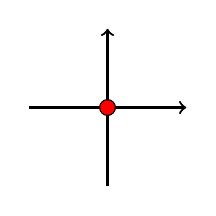
\begin{tikzpicture}
					\draw[->,thick] (-1,0) -- (1,0);
					\draw[->,thick] (0,-1) -- (0,1);
					\draw[fill=red] (0,0) circle (0.1);
				\end{tikzpicture}
			\end{center}
			\item \itemEq{k=1,r=2:\left\lbrace x\in\real^2\mid \left( \frac{x_1}{a_1}\right)^2-\left( \frac{x_2}{a_2}\right)^2=0\right\rbrace\notag}
			\begin{center}
				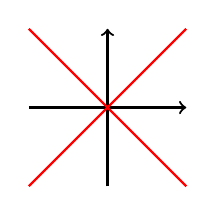
\begin{tikzpicture}
				\draw[->,thick] (-1,0) -- (1,0);
				\draw[->,thick] (0,-1) -- (0,1);
				\draw[thick, red] (-1,-1) -- (1,1);
				\draw[thick, red] (-1,1) -- (1,-1);
				\end{tikzpicture}
			\end{center}
			\item \itemEq{k=1,r=1:\left\lbrace x\in\real^2\mid \left( \frac{x_1}{a_1}\right)^2=0\right\rbrace\notag}
			\begin{center}
				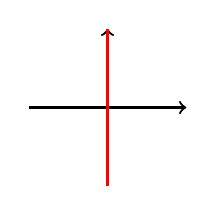
\begin{tikzpicture}
				\draw[->,thick] (-1,0) -- (1,0);
				\draw[->,thick] (0,-1) -- (0,1);
				\draw[thick, red] (0,-1) -- (0,1);
				\end{tikzpicture}
			\end{center}
		\end{itemize}
		\item \begin{itemize}
			\item\itemEq{k=2,r=2:\left\lbrace x\in\real^2\mid \left( \frac{x_1}{a_1}\right)^2+\left( \frac{x_2}{a_2}\right)^2=1 \right\rbrace\notag}
			\begin{center}
				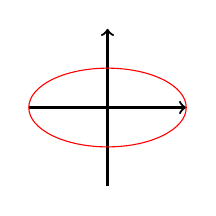
\begin{tikzpicture}
					\draw[->,thick] (-1,0) -- (1,0);
					\draw[->,thick] (0,-1) -- (0,1);
					\draw[red] (0,0) ellipse (1cm and 0.5cm);
				\end{tikzpicture}
			\end{center}
			\item\itemEq{k=1,r=2:\left\lbrace x\in\real^2\mid \left( \frac{x_1}{a_1}\right)^2-\left( \frac{x_2}{a_2}\right)^2=1 \right\rbrace\notag}
			\begin{center}
				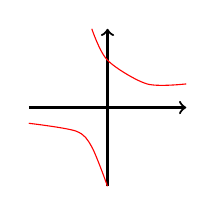
\begin{tikzpicture}
					\draw[->,thick] (-1,0) -- (1,0);
					\draw[->,thick] (0,-1) -- (0,1);
					\draw[red] plot [smooth] coordinates {(-0.2,1) (0,0.6) (0.5,0.3) (1,0.3)};
					\draw[red] plot [smooth] coordinates {(-1,-0.2) (-0.4,-0.3) (-0.2,-0.5) (0,-1)};
				\end{tikzpicture}
			\end{center}
			\item\itemEq{k=1,r=1:\left\lbrace x\in\real^2\mid \left( \frac{x_1}{a_1}\right)^2=1 \right\rbrace\notag}
			\begin{center}
				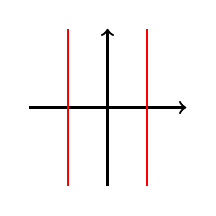
\begin{tikzpicture}
				\draw[->,thick] (-1,0) -- (1,0);
				\draw[->,thick] (0,-1) -- (0,1);
				\draw[thick, red] (-0.5,-1) -- (-0.5,1);
				\draw[thick, red] (0.5,-1) -- (0.5,1);
				\end{tikzpicture}
			\end{center}
			\item\itemEq{k=0,r=2:\left\lbrace x\in\real^2\mid -\left( \frac{x_1}{a_1}\right)^2-\left( \frac{x_2}{a_2}\right)^2=1 \right\rbrace=\emptyset\notag}
			\item\itemEq{k=0,r=1:\left\lbrace x\in\real^2\mid -\left( \frac{x_1}{a_1}\right)^2-\left( \frac{x_2}{a_2}\right)^2=1 \right\rbrace=\emptyset\notag}
		\end{itemize}
		\item \begin{itemize}
			\item\itemEq{k=1,r=1:\left\lbrace x\in\real^2\mid \left( \frac{x_1}{a_1}\right)^2-2x_2=0 \right\rbrace \notag}
			\begin{center}
				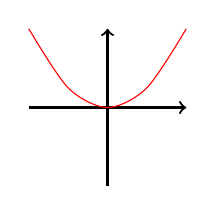
\begin{tikzpicture}
					\draw[->,thick] (-1,0) -- (1,0);
					\draw[->,thick] (0,-1) -- (0,1);
					\draw[red] plot [smooth] coordinates {(-1,1) (-0.5,0.25) (0,0) (0.5,0.25) (1,1)};
				\end{tikzpicture}
			\end{center}
		\end{itemize}
	\end{itemize}
\end{example}

\begin{remark}
	\begin{itemize}
		\item Ist $Q\subseteq\real^2$ eine Quadrik, $U\subseteq V$ affiner Untervektorraum, so ist $Q\cap U$ eine Quadrik in dem Sinne, dass $\exists f\text{ Isometrie}: f(U)=\real^k$ und $f(Q\cap U)$ ist eine Quadrik.
		\item Ebene Quadriken sind im wesentlichen Kegelschnitte, $Q'=\{x\in\real^3\mid x_1^2+x_2^2=x_3^2\}$, außer 2c und 2d in \propref{6_8_example}
	\end{itemize}
\end{remark}

\begin{remark}
	Die Situation wird deutlich übersichtlicher, wenn man den affinen Raum $\real^n$ durch Hinzunahme von Punkten im Unendlichen zum \begriff{projektiven Raum} $\mathbb{P}^n(\real)$ vervollstädigt und den Abschluss der Quadriken darin betrachtet. Es stellt sich dann heraus, dass vom projektiven Standpunkt aus die meisten ebenen Quadriken ähnlich aussehen. (Siehe Vorlesung \textit{Elementare Algebraische Geometrie})
\end{remark}


\chapter{Dualität}
\section{Das Lemma von Zorn}

Sei $K$ ein Körper und $U,V,W$ seien $K$-Vektorräume. Zudem sei $X$ eine Menge.

\begin{definition}[Relation]
	Eine \begriff{Relation} ist eine Teilmenge $R\subseteq X\times X$. Man schreibt $(x,x')\in R$ als $xRx'$. $R$ heißt
	\begin{itemize}
		\item \begriff[Relation!]{reflexiv}, wenn $\forall  x\in X$: $xRx$
		\item \begriff[Relation!]{transitiv}, wenn $\forall x,y,z\in X$: $xRy$ und $yRz\Rightarrow xRz$
		\item \begriff[Relation!]{symmetrisch}, wenn $\forall x,y\in X$: $xRy\Rightarrow yRx$
		\item \begriff[Relation!]{antisymmetrisch}, wenn $\forall x,y\in X$: $xRy$ und $yRx\Rightarrow y=x$
		\item \begriff[Relation!]{total}, wenn $\forall x,y\in X$: $(x,y)\notin R\Rightarrow (y,x)\in R$
	\end{itemize}
\end{definition}

\begin{definition}[Äquivalenzrelation]
	Eine \begriff{Äquivalenzrelation} ist eine reflexive, transitive und symmetrische Relation.
\end{definition}

\begin{definition}[Halbordnung]
	Eine \begriff{Halbordnung} ist eine reflexiv, transitive und antisymmetrische Relation. Eine totale Halbordnung heißt \begriff{Totalordnung} oder \begriff{lineare Ordnung}
\end{definition}

\begin{example}
	\begin{itemize}
		\item Die natürliche Ordnung auf $\real$, $\ratio$, $\whole$ und $\natur$.
		\item Teilbarkeit ist eine Halbordnung auf $\natur$, aber Teilbarkeit ist keine Halbordnung auf $\whole$, da $1\vert -1$ und $-1\vert 1$, aber $1\neq -1$!
		\item $\mathcal{P}(X)$ ist die Potenzmenge. "'$\subseteq$"' ist eine Halbordnung auf $\mathcal{P}$, aber für $\vert X\vert>1$ ist "'$\subseteq$"' keine Totalordnung.
		\item Sei $(X,\le)$ eine Halbordnung, sei $Y\subseteq X$, so ist $(Y,\subseteq\vert_Y)$ eine Halbordnung.
	\end{itemize}
\end{example}

\begin{definition}[Kette]
	Sei $(X,\le)$ eine Halbordnung, $Y\subseteq X$. $Y$ heißt \begriff{Kette}, wenn $(Y,\le\vert_Y)$ total ist.
	
	$x\in Y$ heißt ein \begriff[Kette!]{minimales Element} von $Y$, wenn $\forall x'\in Y$: $x<x'$.
	
	$x\in Y$ heißt \begriff[Kette!]{untere Schranke} von $Y$, wenn $\forall y\in Y$: $y\ge x$.
	
	$x\in Y$ heißt \begriff[Kette!]{kleinstes Element} von $Y$, wenn $x$ untere Schranke von $Y$ ist.
	
	Analog: \begriff[Kette!]{maximales Element}, \begriff[Kette!]{obere Schranke}, \begriff[Kette!]{größtes Element}.
\end{definition}

\begin{center}
	\begin{tikzpicture}
		\node[place] (A) {1};
		\node[place] (B) [below=of A] {3};
		\node[place] (C) [left=of B] {2};
		\node[place] (D) [right=of B] {5};
		\node[place] (E) [right=of D] {7};
		\node[place] (dots) [right=of E] {...};
		
		\node[place] (F) [below=of C] {4};
		\node[place] (G) [below=of B] {6};
		\node[place] (H) [below=of E] {15};
		\node[place] (I) [right=of G] {10};
		\node[place] (dots2) [right=of H] {...};
		
		\node[place] (J) [below=of F] {8};
		\node[place] (K) [below=of J] {16};
		\node[place] (L) [below=of K] {32};
		
		\draw[->,thick] (A.west) -- (C.north);
		\draw[->,thick] (A.south) -- (B.north);
		\draw[->,thick] (A.east) -- (D.north);
		\draw[->,thick] (A.east) -- (E.north);
		\draw[->,thick] (A.east) -- (dots.north);
		
		\draw[->,thick] (C.south) -- (F.north);
		\draw[->,thick] (C.south) -- (G.north);
		\draw[->,thick] (B.south) -- (G.north);
		\draw[->,thick] (C.south) -- (I.north);
		\draw[->,thick] (D.south) -- (I.north);
		\draw[->,thick] (B.south) -- (H.north);
		\draw[->,thick] (D.south) -- (H.north);
		\draw[->,thick] (E.south) -- (dots2.north);
		\draw[->,thick] (D.south) -- (dots2.north);
		
		\draw[->,thick] (F.south) -- (J.north);
		\draw[->,thick] (J.south) -- (K.north);
		\draw[->,thick] (K.south) -- (L.north);
	\end{tikzpicture}
	$Y=\{2^n\mid n\in\natur\}$ ist eine Kette
\end{center}

\begin{remark}
	\begin{itemize}
		\item Hat $Y$ ein kleinstes Element, so ist dies eindeutig bestimmt. Ein kleinstes Element ist minimal.
		\item Jede endliche Halbordnung hat minimale Elemente. Jede endliche Totalordnung hat ein kleinstes Element. Analog für maximale Elemente und größtes Element.
	\end{itemize}
\end{remark}

\begin{example}
	$(\natur,\le)$ hat als kleinstes Element die 1, aber kein größtes Element oder maximale Elemente.
\end{example}

\begin{example}
	$V=\real^3$, $\mathcal{X}$ die Menge der Untervektorräume des $\real^3$. $(\mathcal{X},\le)$ ist eine Halbordnung auf $Y\subseteq X$ mit $Y=\{U\in\mathcal{X}\mid \dim_\real(U)\le 2\}$. 
	\begin{itemize}
		\item $Y$ hat ein kleinstes Element: $\{0\}$.
		\item Es gibt unendlich viele maximale Elemente in $Y$, nämlich die Untervektorräume von $V$, die die Dimension 2 haben. Es gibt also kein größtes Element.
		\item $V$ ist die obere Schranke von $Y$.
	\end{itemize}
\end{example}

\begin{theorem}[Das Lemma von Zorn]
	Sei $(X,\le)$ eine Halbordnung, die nicht leer ist. Wenn jede Kette eine obere Schranke hat, dann hat $X$ ein maximales Element.
\end{theorem}
\begin{proof}
	Dieses Theorem ist äquivalent zum Auswahlaxiom. \frownie{}
\end{proof}

\begin{conclusion}
	Zu jeder Familie $(x_i)$, nicht leer, gibt es eine \begriff{Auswahlfunktion}, das heißt eine Abbildung:
	\begin{align}
		f: I\to \bigcup X_i\text{ mit } f(i)\in X_i\quad\forall i\notag
	\end{align}
\end{conclusion}

\section{Der Dualraum}

Sei $V$ ein $K$-Vektorraum.

\begin{definition}[Dualraum]
	Der \begriff{Dualraum} zu $V$ ist der $K$-Vektorraum
	\begin{align}
		V^*=\Hom_K(V,K)=\{\phi:V\to K\text{ linear}\}\notag
	\end{align}
	Die Elemente von $V^*$ heißen \begriff{Linearformen} auf $V$.
\end{definition}

\begin{example}
	Ist $V=K^n=\Mat_{n\times 1}(K)$, so wird $V^*=\Hom_K(V,K)$ durch $\Mat_{1\times n}(K)\cong K^n$. Wir können also die Elemente von $V$ als Spaltenvektoren und die Linearformen auf $V$ als Zeilenvektoren auffassen.
\end{example}

\begin{lemma}
	Ist $B(x_1)_{i\in I}$ eine Basis von $V$, so gibt es zu jedem $i\in I$ genau $x_i^*\in V^*$ mit $x_i^*(x_j)=\delta_{ij}\quad\forall j\in I$.
\end{lemma}
\begin{proof}
	Siehe LAAG1 III.5.1, angewandt auf die Familie $(y_j)_{j\in I}$, $y_j\delta_{i.j}$ in $W=K$. %TODO: Verlinkung
\end{proof}

\begin{proposition}
	Ist $B=(x_1)_{i\in I}$ eine Basis von $V$, so ist $B^*=(x_i^*)_{i\in I}$ linear unabhängig. Ist $I$ endlich, so ist $B^*$ eine Basis von $V^*$.
\end{proposition}
\begin{proof}
	Ist $\phi=\sum_{i\in I} \lambda_ix_i^*$, $\lambda_i\in K$, fast alle gleich 0, so ist $\phi(x_j)=\sum_{i\in I} \lambda_j x_i^*(x_j)=\lambda_j$ für jedes $j\in I$. Ist also $\phi=0$, so ist $\lambda_j=\phi(x_j)=0\quad\forall j\in I$, $B^*$ ist somit linear unabhängig. \\
	Ist zudem $I$ endlich und $\psi\in V^*$, so ist $\psi=\psi'=\sum_{i\in I} \psi(x_i)x_i^*$, denn $\psi'(x_j)=\sum_{i\in I} \psi(x_i)x_i^*(x_j)=\psi(x_i)\quad\forall j\in I$, und somit ist $B^*$ ein Erzeugendensystem von $V^*$.
\end{proof}

\begin{definition}[duale Basis]
	Ist $B=(x_i)_{i\in I}$ eine endliche Basis von $V$, so nennt man $B^*=(x_i^*)_{i\in I}$ die zu $B$ \begriff{duale Basis}.
\end{definition}

\begin{conclusion}
	Zu jeder Basis $B$ von $V$ gibt es einen eindeutig bestimmtem Monomorphismus
	\begin{align}
		f_V\to V^*\text{ mit } f(B)=B^*\notag
	\end{align}
	Ist $\dim_K(V)<\infty$, so ist dieser ein Isomorphismus.
\end{conclusion}

\begin{conclusion}
	Zu jedem $=0\neq x\in V$ gibt es eine Linearform $\phi\in V$ mit $\phi(x)=1$.
\end{conclusion}
\begin{proof}
	Ergänze $x_1=x$ zu einer Basis $(x_i)_{i\in I}$ von $V$ (\propref{3_1_11}) und $\phi=x_1^*$.
\end{proof}

\begin{example}
	Ist $V=K^n$ mit Standardbasis $\mathcal{E}=(e_1,...,e_n)$, so können wir $V^*$ mit dem Vektorraum der Zeilenvektoren identifizieren, und dann ist
	\begin{align}
		e_i^* = e_i^t\notag
	\end{align}
\end{example}

\begin{definition}[Bidualraum]
	Der \begriff{Bidualraum} zu $V$ ist der $K$-Vektorraum
	\begin{align}
		V^{**}=(V^*)^*=\Hom_K(V^*,K)\notag
	\end{align}
\end{definition}

\begin{proposition}
	Die kanonische Abbildung
	\begin{align}
		\iota:\begin{cases}
		V\to V^{**} \\ x\to \iota_x
		\end{cases}\text{ wobei } \iota_x(\phi)=\phi(x)\notag
	\end{align}
	ist ein Monomorphismus. Ist $\dim_K(V)<\infty$, so ist $\iota$ ein Isomorphismus.
\end{proposition}
\section{Die duale Abbildung}

Sei $f\in\Hom_K(V,W)$.

\begin{remark}
	Ist $\phi\in W^*=\Hom_K(W,K)$ eine Linearform auf $W$, so ist $\phi\circ f\in \Hom_K(V,K)=V^*$ eine Linearform auf $V$.
	%TODO: Bild von Pascal
\end{remark}

\begin{center}
	\begin{tikzcd}
		V \arrow[r, "f"] \arrow[dr, dashrightarrow, "f^{\ast}(\phi)"]
		& W \arrow[d, "\phi"]\\
		& K\\
		V^{\ast} & \arrow[l, "f^{\ast}"] W^{\ast}
	\end{tikzcd}
\end{center}

\begin{definition}[duale Abbildung]
	Die zu $f$ duale Abbildung ist
	\begin{align}
		f^*:
		\begin{cases}
			W^*\to V^* \\
			\phi\mapsto \phi\circ f
		\end{cases} \notag
	\end{align}
\end{definition}

\begin{lemma}
	Es ist $f^*\in\Hom_K(W^*,V^*)$.
\end{lemma}
\begin{proof}
	Sind $\phi,\psi\in W^*$ und $\lambda\in K$ ist 
	\begin{align}
		f^*(\phi+\psi) &= (\phi+\psi)\circ f \notag \\
		&= \phi\circ f + \psi\circ f \notag \\
		&= f^*(\phi) + f^*(\psi) \notag \\
		f^*(\lambda\phi) &= (\lambda\phi)\circ f \notag \\
		&= \lambda\cdot(\phi\circ f) \notag \\
		&= \lambda\cdot f^*(\phi) \notag
	\end{align}
\end{proof}

\begin{proposition}
	\proplbl{3_3_4}
	Sind $B=(x_1,...,x_n)$ und $C=(y_1,...,y_m)$ Basen von $V$ bzw. $W$, so ist
	\begin{align}
		M_{B^*}^{C^*}(f^*)=\left(M_C^B(f) \right)^t\notag
	\end{align}
\end{proposition}
\begin{proof}
	Sei $A=M_C^B(f)=(a_{ij})_{i,j}$ und $B=M_{B^*}^{C^{*}}(f^*)=(b_{ji})_{j,i}$. Dann ist $f(x_j)=\sum_{i=1}^m a_{ij}y_i$, also $a_{ji}=y_i^*(f(x_j))=f^*(y_i^*)(x_j)$ und $f^*(y_i^*)=\sum_{j=1}^n b_{ji}x_j^*$, also $b_{ji}=f^*(y_i^*)(x_j)=a_{ij}$.
\end{proof}

\begin{conclusion}
	\proplbl{3_3_5}
	Sind $V$ und $W$ endlichdimensional, und identifizieren wir $V=V^{**}$ und $W=W^{**}$, so ist $f=f^{**}$, das heißt $\iota\circ f=f^{**}\circ\iota$.
	%TODO: Bild von Pascal
	
\end{conclusion}

\begin{center}
	\begin{tikzcd}
		V \arrow[r, "f"] \arrow[d, "\iota_V \cong"] 
		& W \arrow[d, "\iota_W \cong"] \\
		V^{\ast \ast} \arrow[r, "f^{\ast \ast}"] 
		& W^{\ast \ast}
	\end{tikzcd}
\end{center}

\begin{proof}
	Seien $B$ und $C$ Basen von $V$ bzw. $W$. Unter der Identifizierung ist $B^{**}=B$ und $C=C^{**}$, das heißt $\iota(x_i)=x_i^{**}$ bzw. $\iota(y_j)=y_j^{**}$, denn $\iota(x_i)(x_j^*)=x_j^*(x_i)=\delta_{ij} = x_i^{**}(x_j^*)\quad\forall i,j$ und somit 
	\begin{align}
		M_C^B(f^{**}) \overset{\propref{3_3_4}}{=} \left( M_{B^*}^{C^*}(f^*)\right)^t \overset{\propref{3_3_4}}{=} \left( M_C^B(f)\right)^{tt}=M_C^B(f)\notag
	\end{align}
	Also $f^{**}=f$.
\end{proof}

\begin{conclusion}
	Sind $V,W$ endlichdimensional, so liefert die Abbildung $f\mapsto f^*$ einen Isomorphismus von $K$-Vektorräumen.
	\begin{align}
		\Hom_K(V,W)\to \Hom_K(W^*,V^*)\notag
	\end{align}
\end{conclusion}
\begin{proof}
	Sind $f,g\in\Hom_K(V,W)$ und $\lambda\in K$, $\phi\in W^{*}$, so ist
	\begin{align}
		(f+g)^*(\phi)&=\phi\circ(f+g)=\phi\circ f+\phi\circ g=f^*(\phi)+g^*(\phi)=(f^*+g^*)(\phi) \notag \\
		(\lambda f)^*(\phi)&=\phi\circ (\lambda f)=\lambda\cdot(\phi\circ f)=\lambda\circ f^*(\phi)=(\lambda f^*)(\phi)\notag
	\end{align}
	Die Abbildung ist somit linear. Nach \propref{3_3_5} ist sie injektiv. Da 
	\begin{align}
		 \dim_K(V,W)&=\dim_K(V)\cdot \dim_K(W)\notag \\
		 &=\dim_K(V^*)\cdot \dim_K(W^*) \notag \\
		 &= \dim_K(\Hom_K(W^*,V^*))\notag
	\end{align}
	ist sie auch ein Isomorphismus.
\end{proof}

\begin{proposition}
	\proplbl{3_3_7}
	Sind $V,W$ endlichdimensional so ist
	\begin{align}
		\Image(f^*)&=\Ker(f)^0\notag \\
		\Ker(f^*)&=\Image(f)^0\notag
	\end{align}
\end{proposition}
\begin{proof}
	\begin{itemize}
		\item $\Image(f^*)\subseteq\Ker(f)^0$: Ist $\phi\in W^*$, $x\in \Ker(f)$, so ist
		\begin{align}
			f^*(\phi)(x)=(\phi\circ f)(x)=\phi(0)=0\notag
		\end{align}
		\item $\Ker(f)^0\subseteq\Image(f^*)$: Sei $\phi\in\Ker(f)^0$. Setze eine Basis $(x_1,...,x_r)$ von $\Ker(f)$ zu einer Basis $(x_1,...,x_n)$ von $V$ fort. Dann sind $f(x_{r+1}),...,f(x_n)$ linear unabhängig nach der Kern-Bild-Formel (LAAG 1 III.7.13), es gibt also $\psi\in W^*$ mit 
		\begin{align}
			\psi(f(x_i))=\phi(x_i)\quad\forall i\notag
		\end{align}
		Es folgt
		\begin{align}
			f^*(\psi)(x_i)=\psi(f(x_i))=\phi(x_i)\quad\forall i\notag
		\end{align}
		also $\phi=f^*(\psi)$. %TODO: Verlinkung
		\item Mit der Identifizierung $V=V^{**}$ ist
		\begin{align}
			\Image(f)^0\overset{\propref{3_3_5}}{=}\Image(f^{**})^0=\Ker(f^*)^{00}\overset{\propref{3_2_15}}{=}\Ker(f^*)\notag
		\end{align}
	\end{itemize}
\end{proof}

\begin{conclusion}
	Sind $V,W$ endlichdimensional, so ist
	\begin{align}
		\rk(f)=\rk(f^*)\notag
	\end{align}
\end{conclusion}
\begin{proof}
	\begin{align}
		\rk(f) &= \dim_K(\Image(f))\notag \\
		&\overset{\propref{3_2_14}}{=} \dim_K(W)-\dim_K(\Image(f)^0)\notag \\
		&\overset{LAAG1.III.7.13}{=} \dim_K(W^*)-\dim_K(\Ker(f^*)) \notag \\
		&= \rk(f^*)\notag %TODO: Verlinkung
	\end{align}
\end{proof}

\begin{conclusion}
	\proplbl{3_3_9}
	Ist $\dim_K(V)<\infty$ und $U\subseteq V$ ein Untervektorraum, so lässt sich jede Linearform auf $U$ zu einer Linearform auf $V$ fortsetzen.
\end{conclusion}
\begin{proof}
	Ist $f:U\to V$ die Inklusionsabbildung, so ist $f^*:V^*\to U^*$, $\phi\mapsto\phi\vert_U$ und
	\begin{align}
		\rk(f^*)=\rk(f)=\dim_K(U)=\dim_K(U^*)\notag
	\end{align}
	$f^*$ ist somit surjektiv.
\end{proof}

\begin{remark}
	\propref{3_3_9} gilt auch ohne die Voraussetzung $\dim_K(V)<\infty$, siehe Übung.
\end{remark}

\begin{remark}
	Ein homogenes lineares Gleichungssystem $Ax=0$ hat als Lösungsraum $L(A,0)\subseteq K^n$ ein Untervektorraum des $K^n$. Unter der Identifizierung $K^n=(K^n)^{**}$ ist $L(A,0)$ der Annulator der Linearformen beschrieben durch die Zeilen $a_1,...,a_m\in (K^n)^*$ von $A$. Wir wollen umgekehrt zu einem Untervektorraum $W\subseteq K^n$ ein $A=(a_1,...,a_m)\in\Mat_{n\times m}(K)$ mit $W=L(A,0)$ finden. Ist $W=\Span_K(b_1,...,b_r)$, so ist $W=\Image(f_B)$ mit $B=(b_1,...,b_r)\in\Mat_{n\times r}(K)$. \\
	$\Rightarrow W\overset{\propref{3_3_7}}{=}\Ker(f^*_B)^0$ und $M_{\mathcal{E}^t}(f^*_B)=B^t$. Wenn man also eine Basis $(a_1,...,a_s)$ von $L(B^t,0)$ bestimmt und daraus eine Matrix $A=(a_1^t,...,a_s^t)\in\Mat_{s\times n}(K)$ bildet, so ist $W=L(A,0)$.
\end{remark}
\section{Die adjungierte Abbildung}

Sei $K=\real$ oder $K=\comp$ und $V$ ein endlichdimensionaler unitärer $K$-Vektorraum.

\begin{definition}[weitere Skalarmultiplikation]
	Wir definieren auf $V$ eine Skalarmultiplikation
	\begin{align}
		\lambda\ast x=\overline{\lambda}\cdot x\notag
	\end{align}
	und schreiben $\overline{V}=(V,+,\ast)$.
\end{definition}

\begin{lemma}
	$\overline{V}$ ist ein $K$-Vektorraum und $\End_K(V)=\End_K(\overline{V})$.
\end{lemma}
\begin{proof}
	Mit LAAG1 VI.1.7 nachprüfen, zum Beispiel:
	\begin{itemize}
		\item $\lambda\ast (x+y)=\overline{\lambda}\cdot (x+y)=\overline{\lambda} x+\overline{\lambda} y=\lambda\ast x+\lambda\ast y$
		\item $\lambda\ast(\mu\ast x)=\overline{\lambda}(\overline{\mu}\cdot x)=\overline{\lambda\mu}x=(\lambda\mu)\ast x$
	\end{itemize}
	Weiterhin sei: $f\in\End_K(V)$, $x\in V$, $\lambda\in K$ \\
	$\Rightarrow f(\lambda\ast x)=f(\overline{\lambda}x)=\lambda\ast f(x)$ \\
	$\Rightarrow f\in \End_K(\overline{V})$. \\
	Umgekehrt sei $g\in\End_K(\overline{V})$, $x\in V$, $\lambda\in K$ \\
	$\Rightarrow g(\lambda\cdot x)=g(\overline{\lambda}\ast x)=\lambda\cdot g(x)$ \\
	$\Rightarrow g\in \End_K(V)$. \\
\end{proof}

\begin{lemma}
	Für $y\in V$ ist
	\begin{align}
		\Phi_y:
		\begin{cases}
			V\to K \\ x\mapsto\skalar{x}{y}
		\end{cases}\notag
	\end{align}
	eine Linearform auf $V$.
	
	Die Abbildung $y\mapsto\Phi_y$ liefert einen Isomorphismus $\Phi:\overline{V}\to V^*$.
\end{lemma}
\begin{proof}
	\begin{itemize}
		\item $\Phi_y\in V^*$: Linearität in ersten Argument.
		\item $\Phi\in \Hom_K(\overline{V},V^*)$: Für $y,y'\in V$, $\lambda\in K$, $x\in V$ ist
		\begin{itemize}
			\item $\Phi_{y+y'}(x)=\skalar{x}{y+y'}=\skalar{x}{y}+\skalar{x}{y'}=\Phi_y(x)+\Phi_{y'}(x)$
			\item $\Phi_{\lambda\ast y}(x)=\skalar{x}{\lambda\ast x}=\skalar{x}{\overline{\lambda}y}=\lambda \skalar{x}{y}=\lambda\Phi_y(x)$
		\end{itemize}
		\item $\Phi$ injektiv: Skalarprodukt ist nicht ausgeartet.
		\item Da $\dim_K(\overline{V})=\dim_K(V)=\dim_K(V^*)$ ist $\Phi$ somit ein Isomorphismus.
	\end{itemize}
\end{proof}

\begin{proposition}
	Zu $f\in\End_K(V)$ gibt es ein eindeutig bestimmtes $f^{adj}\in\End_K(V)$ mit 
	\begin{align}
		\skalar{f(x)}{y}=\skalar{x}{f^{adj}(y)}\quad\forall x,y\in V\notag
	\end{align}
\end{proposition}
\begin{proof}
	
\end{proof}

\begin{definition}[adjungierter Endomorphismus]
	Die Abbildung $f^{adj}$ heißt der zu $f$ \begriff[Endomorphismus!]{adjungierte Endomorphismus}.
\end{definition}

\begin{example}
	\begin{itemize}
		\item Ist $f$ selbstadjungiert, so ist $f^{adj}=f$.
		\item Ist $f$ unitär, so ist $f\in\Aut_K(V)$ und 
		\begin{align}
		\skalar{f(x)}{y}=\skalar{x}{f^{-1}(y)}\quad\forall x,y\in V\notag
		\end{align}
		also $f^{adj}=f^{-1}$.
	\end{itemize}
\end{example}
\section{Der Spektralsatz}

Sei $V$ ein endlichdimensionaler unitärer $K$-Vektorraum und $f\in\End_K(V)$.

\begin{definition}[normaler Endomorphismus, normale Matrix]
	Der Endomorphismus $f$ heißt \begriff[Endomorphismus!]{normal}, wenn
	\begin{align}
		f\circ f^{adj}=f^{adj}\circ f\notag
	\end{align}
	
	Entsprechend heißt $A\in\Mat_n(K)$ \begriff[Matrix!]{normal}, wenn
	\begin{align}
		AA^*=A^*A\notag
	\end{align}
\end{definition}

\begin{mathematica}[normale Matrix]
	Ob eine Matrix $A$ normal ist, beantwortet folgende Funktion für Mathematica bzw. WolframAlpha:
	\begin{align}
		\texttt{NormalMatrixQ[A]}\notag
	\end{align}
\end{mathematica}

\begin{example}
	\begin{itemize}
		\item Ist $f$ selbstadjungiert, so ist $f^{adj}=f$, insbesondere ist $f$ normal.
		\item Ist $f$ unitär, so ist $f^{adj}=f^{-1}$, insbesondere ist $f$ normal.
	\end{itemize}
\end{example}

\begin{lemma}
	\proplbl{7_5_3}
	Genau dann ist $f\in\End_K(V)$ normal, wenn
	\begin{align}
		\skalar{f(x)}{f(y)}=\skalar{f^{adj}(x)}{f^{adj}(y)}\quad\forall x,y\in V\notag
	\end{align}
\end{lemma}
\begin{proof}
	\begin{itemize}
		\item Hinrichtung: Ist $f$ normal, so ist
		\begin{align}
			\skalar{f(x)}{f(y)} &= \skalar{x}{(f^{adj}\circ f)(y)} \notag \\
			&= \skalar{x}{(f\circ f^{adj})(y)} \notag \\
			&= \skalar{f^{adj}(x)}{f^{adj}(y)}\quad\forall x,y\in V\notag
		\end{align}
		\item Rückrichtung: Ist umgekehrt $\skalar{f^{adj}(x)}{f^{adj}(y)}$, so ist
		\begin{align}
			\skalar{x}{(f^{adj}\circ f)(y)}&=\skalar{x}{(f\circ f^{adj})(y)} \notag \\
			0 &= \skalar{x}{(f^{adj}\circ f-f\circ f^{adj})(y)} \notag \\
			f^{adj}\circ f&=f\circ f^{adj} \notag
		\end{align}
	\end{itemize}
\end{proof}

\begin{lemma}
	\proplbl{7_5_4}
	Ist $f$ normal, ist ist
	\begin{align}
		\Ker(f)=\Ker(f^{adj})\notag
	\end{align}
\end{lemma}
\begin{proof}
	Nach \propref{7_5_3} ist
	\begin{align}
		\Vert f(x)\Vert = \Vert f^{adj}(x)\Vert \quad\forall x\in V\notag
	\end{align}
	Insbesondere gilt
	\begin{align}
		f(x)=0\iff f^{adj}(x)=0\notag
	\end{align}
\end{proof}

\begin{lemma}
	\proplbl{7_5_5}
	Ist $f$ normal, so ist
	\begin{align}
		\Eig(f,\lambda)=\Eig(f^{adj},\overline{\lambda})\quad\forall\lambda\in K\notag
	\end{align}
\end{lemma}
\begin{proof}
	Da $(\lambda\cdot \id-f)^{adj}\overset{\propref{7_4_8}}{=}\overline{\lambda}\cdot\id-f^{adj}$ ist auch $\lambda\cdot\id-f$ normal. Somit ist
	\begin{align}
		\Eig(f,\lambda) &= \Ker(\lambda\id-f)\notag \\
		&\overset{\propref{7_5_4}}{=} \Ker((\lambda\id-f)^{adj})\notag \\
		&= \Ker(\overline{\lambda}\id-f^{adj})\notag \\
		&= \Eig(f^{adj},\overline{\lambda})\notag
	\end{align}
\end{proof}

\begin{theorem}[Spektralsatz]
	\proplbl{7_5_6}
	Sei $f\in\End_K(V)$ ein Endomorphismus, für den $\chi_f$ in Linearfaktoren zerfällt. Genau dann besitzt $V$ eine Orthonormalbasis aus Eigenvektoren von $f$, wenn $f$ normal ist.
\end{theorem}
\begin{proof}
	\begin{itemize}
		\item Hinrichtung: Ist $B$ eine Orthonormalbasis aus Eigenvektoren von $f$, so ist $A=M_B(f)$ eine Diagonalmatrix. Dann ist auch $M_B(f^{adj})\overset{\propref{7_4_7}}{=}A^*$ eine Diagonalmatrix und $AA^*=A ^*A$. Somit ist $f$ normal.
		\item Rückrichtung: Sei $f$ normal und $\chi_f(t)=\prod_{i=1}^n (t-\lambda_i)$. Beweis nach Induktion nach $n=\dim_K(V)$. \\
		\emph{$n=0$}: klar \\
		\emph{$n-1\to n$}: Wähle Eigenvektor zum Eigenwert $\lambda_1$, o.E. $\Vert x_1\Vert = 1$. Sei $U=K\cdot x_1$. Nach \propref{7_5_5} ist $f^{adj}(x_1)=\overline{\lambda_1}x_1$, insbesondere ist $U$ $f$-invariant und $f^{adj}$-invariant. Für $x\in U^\perp$ ist 
		\begin{align}
			\skalar{f(x)}{x_1}= \skalar{x}{f^{adj}(x_1)}=\skalar{x}{\overline{\lambda_1}x_1}=\lambda_1\skalar{x}{x_1}=0\notag
		\end{align}
		also $f(x)\in U^\perp$ und 
		\begin{align}
			\skalar{f^{adj}(x)}{x_1}=\skalar{x}{f(x_1)}=\skalar{x}{\lambda_1 x_1}=\overline{\lambda_1} \skalar{x}{x_1}=0\notag
		\end{align}
		also $f^{adj}(x)\in U^\perp$. Somit ist $V=U\oplus U^\perp$ eine Zerlegung in Untervektorräume, die sowohl $f$-invariant als auch $f^{adj}$-invariant sind. Insbesondere st $f^{adj}\vert_{U^\perp}=(f\vert_{U^\perp})^{adj}$, woraus folgt, dass auch $f\vert_{U^\perp}$ normal ist:
		\begin{align}
			f\vert_{U^\perp}\circ (f\vert_{U^\perp})^{adj}=f\circ f^{adj}\vert_{U^\perp}=f^{adj}\circ f\vert_{U^\perp} = f^{adj}\vert_{U^\perp}\circ f\vert_{U^\perp}=(f\vert_{U^\perp})^{adj}\circ f\vert_{U^\perp}\notag
		\end{align}
		Außerdem zerfällt auch $\chi_{f\vert_{U^\perp}}=\prod_{i=2}^n (t-\lambda_i)$ in Linearfaktoren. Nach Induktionshypothese existiert eine Orthonormalbasis $(x_2,...,x_n)$ von $U^\perp$ bestehend aus Eigenvektoren von $f\vert_{U^\perp}$ und $(x_1,...,x_n)$ ist dann eine Orthonormalbasis von $V$ aus Eigenvektoren von $f$.
	\end{itemize}
\end{proof}

\begin{conclusion}
	Sei $A\in\Mat_n(\comp)$. Genau dann gibt es $S\in\Uni_n$ mit $S^*AS=D$ eine Diagonalmatrix, wenn $A$ normal ist.
\end{conclusion}

\begin{remark}
	\propref{7_5_6} ist eine gemeinsame Verallgemeinerung von \propref{6_5_9} und \propref{6_6_5}
\end{remark}
\section{Tensorprodukte}

\begin{definition}[billineare Abbildung]
	Eine Abbildung $\xi:V\times W\to U$ ist \begriff[Abbildung!]{bilinear}, wenn für jedes $v\in V$ die Abbildung 
	\begin{align}
		\begin{cases}
		W\to U \\ w\mapsto \xi(v,w)
		\end{cases}\notag
	\end{align}
	und für jedes $w\in W$ die Abbildung
	\begin{align}
	\begin{cases}
	V\to U \\ v\mapsto \xi(v,w)
	\end{cases}\notag
	\end{align}
	linear sind.
	
	Wir definieren
	\begin{align}
		\Bil_K(V,W,U)=\{\xi\in\Abb(V\times W,U)\mid \xi\text{ bilinear}\}\notag
	\end{align}
\end{definition}

\begin{definition}[Tensorprodukt]
	Ein \begriff{Tensorprodukt} von $V$ und $W$ ist ein Paar $(T,\tau)$ bestehend aus einem $K$-Vektorraum $T$ und einer bilinearen Abbildung $\tau\in\Bil_K(V,W,T)$ welche die folgende \begriff{universelle Eigenschaft} erfüllt: \\
	\textit{Ist $U$ ein weiterer $K$-Vektorraum und $\xi\in\Bil_K(V,W,U)$ so gibt es genau ein $\xi_\otimes\in\Hom_K(T,U)$ mit $\xi=\xi_\otimes\circ\tau$.}
	\begin{center}
		\begin{tikzpicture}
		\matrix (m) [matrix of math nodes,row sep=3em,column sep=4em,minimum width=2em]
		{V\times W & T \\ \; & U \\};
		\path[-stealth]
		(m-1-1) edge node [below] {$\xi$} (m-2-2)
		edge node [above] {$\tau$} (m-1-2)
		(m-1-2) edge [dashed] node [right] {$\xi_\otimes$} (m-2-2);
		\end{tikzpicture}
	\end{center}
\end{definition}

\begin{definition}[Vektorraum mit Basis $X$]
	\proplbl{7_6_8}
	Sei $X$ eine Menge. Der $K$-\begriff{Vektorraum mit Basis $X$} ist der Untervektorraum $V=\Span_K((\delta_x)_{x\in X})$ des $K$-Vektorraum $\Abb(X,K)$ mit $\delta_x(y)=\delta_{x,y}=\begin{cases}1&x=y\\0&x\neq y\end{cases}$
\end{definition}

\chapter{Moduln}
In diesem ganzen Kapitel sei $R$ ein kommutativer Ring mit Einselement.

\section{Moduln}

\begin{definition}
	Ein $R$-\begriff{Modul} ist ein Tripel $(M,+,\cdot)$ bestehend aus einer Menge $M$, einer Verknüpfung $+:M\times M\to M$ und der Abbildung $\cdot:R\times M\to M$ (Skalarmultiplikation) für die gelten:
	\begin{itemize}
		\item (M1): $(M,+)$ ist eine abelsche Gruppe
		\item (M2): Addition und Skalarmultiplikation sind verträglich. Für alle $x,y\in M$ und $a,b\in R$ gelten
		\begin{enumerate}
			\item $a(x+y)=ax+ay$
			\item $(a+b)x=ax+bx$
			\item $a\cdot bx=ab\cdot x$
			\item $1\cdot x=x$
		\end{enumerate}
	\end{itemize}
\end{definition}

\begin{example}
	\begin{enumerate}
		\item Ist $R=K$ ein Körper, so sind die $R$-Moduln genau die $K$-Vektorräume.
		\item Ist $R=\whole$, so sind die $R$-Moduln genau die abelschen Gruppen mit der einzig möglichen Skalarmultiplikation 
		\begin{align}
			\whole\times A\to A,(k,a)\mapsto ka=\underbrace{1+...+1}_{k\text{-mal}}a=\underbrace{a+...+a}_{k\text{-mal}}\notag
		\end{align}
		vergleiche Laag 1 III.2.3 %TODO: Verlinkung
		\item Jedes Ideal $M\subseteq R$ ist ein $R$-Modul mit Einschränkung der Multiplikation als Skalarmultiplikation.
		\item Ist $K$ ein Körper, $V$ ein $K$-Vektorraum und $f\in\End_K(V)$, so wird $V$ durch $P(t)\cdot x:=P(f)(x)$ zu einem Modul über dem Ring $R=K[t]$, siehe auch V.5.2 %TODO: Verlinkung
	\end{enumerate}
\end{example}

\begin{definition}[Homomorphismus von $R$-Moduln]
	Seien $M,M'$ $R$-Moduln. Eine Abbildung $f:M\to M'$ ein \begriff[Modul!]{Homomorphismus} von $R$-Moduln (oder $R$-Homomorphismus oder $R$-linear), wenn
	\begin{align}
		f(x+y)&=f(x)+f(y) \notag \\
		f(ax) &= a\cdot f(x)\notag
	\end{align}
	Wir bezeichnen die Menge der $R$-Homomorphismen $f:M\to M'$ mit $\Hom_R(M,M')$. Wie üblich definiert man den \begriff[Modul!]{Kern} eines $R$-Homomorphismus, sowie die Begriffe \begriff[Modul!]{Monomorphismus}, \begriff[Modul!]{Epimorphismus}, \begriff[Modul!]{Isomorphismus}, \begriff[Modul!]{Endomorphismus} und \begriff[Modul!]{Automorphismus} von $R$-Moduln.
\end{definition}

\begin{definition}[Untermodul, Erzeugendensystem]
	Ein \begriff{Untermodul} ist eine nichtleere Teilmenge $N\subseteq M$, für die gilt:
	\begin{itemize}
		\item Sind $x,y\in N$, so ist auch $x+y\in N$.
		\item Ist $a\in R$ und $x\in N$, so ist auch $ax\in N$.
	\end{itemize}

	Für eine Familie $(x_i)_{i\in I}$ ist
	\begin{align}
		\sum_{i\in I} Rx_i=\{\sum_{i\in I} ax_i\mid a\in R\text{, fast alle gleich 0}\}\notag
	\end{align}
	der von $(x_i)_{i\in I}$ \begriff[Untermodul!]{erzeugte Untermodul} von $M$. Ist $\sum_{i\in I} Rx_i=M$, so ist $(x_i)_{i\in I}$ ein \begriff[Modul!]{Erzeugendensystem} von $M$. Der $R$-Modul $M$ ist \begriff[Modul!]{endlich erzeugt}, wenn er ein endliches Erzeugendensystem besitzt.
\end{definition}

\begin{definition}[freie Familie, Basis]
	Eine Familie $(x_i)_{i\in I}$ in $M$ ist \begriff[Familie!]{frei} oder ($R$-linear unabhängig), wenn es keine Familie $(\lambda_i)_{i\in I}$ von Elementen von $R$, fast alle gleich 0, aber nicht alle gleich 0, mit $\sum_{i\in I} \lambda_ix_i=0$ gibt.
	
	Ein freies Erzeugendensystem heißt \begriff[Modul!]{Basis}. Besitzt $M$ eine Basis, so nennt man $M$ \begriff[Modul!]{frei}.
\end{definition}

\begin{definition}[Summen von Moduln]
	Die \begriff[Modul!]{Summe} einer Familie $(N_i)_{i\in I}$ von Untermoduln von $M$ ist
	\begin{align}
		\sum_{i\in I} N_i=\left\lbrace \sum_{i\in I} x_i\mid x_i\in N_i\text{, fast alle gleich 0}\right\rbrace \notag
	\end{align}
	Lässt sich jedes $x\in\sum_{i\in I} N_i$ eindeutig als $\sum_{i\in I} x_i$ mit $x_i\in N_i$ schreiben, so nennt man die Summe \begriff[Modul!]{direkt} und schreibt dafür auch $\bigoplus_{i\in I} N_i$.
	
	Ist $(M_i)_{i\in I}$ eine Familie von $R$-Moduln, so definiert man deren \begriff[Modul!]{(externe) direkte Summe} als das $R$-Modul 
	\begin{align}
		\bigoplus_{i\in I} M_i := \left\lbrace (x_i)_{i\in I}\in \prod_{i\in I} M_i\mid x_i=0\text{ für fast alle } i\in I\right\rbrace \notag
	\end{align}
	mit komponentenweiser Addition und Skalarmultiplikation.
\end{definition}

\begin{definition}[Torsionsmodul]
	Für $a\in R$ definiert man den $a$-\begriff{Torsionsmodul} von $M$ als
	\begin{align}
		M[a]:=\{x\in M\mid ax=0\}\notag
	\end{align}
	Die Elemente des Torsionsmoduls
	\begin{align}
		M_{tor}:=\bigcup_{0\neq a\in R} M[a]=\{x\in M\mid ax=0\text{ für ein } a\in R\backslash\{0\}\}\notag
	\end{align}
	nennt man die \begriff{Torsionselemente} von $M$.
\end{definition}
\section{Teilbarkeit}

\begin{definition}[Teilbarkeit]
	Seien $a,b\in R$.
	\begin{enumerate}
		\item $a$ \begriff{teilt} $b$ (in Zeichen $a\mid b$): Es existiert $x\in R$ mit $b=ax$.
		\item $a$ und $b$ sind \begriff{assoziiert} (in Zeichen $a\sim b$): Es existiert $x\in R^{\times}$ mit $b=ax$.
	\end{enumerate}
\end{definition}

\begin{definition}[größter gemeinsamer Teiler, kleinstes gemeinsames Vielfaches]
	Seien $a,b\in R$. Ein $c\in R$ ist ein \begriff{größter gemeinsamer Teiler} von $a$ und $b$ in Zeichen $c=\ggT(a,b)$, wenn gilt: $c\mid a$ und $c\mid b$ und ist $d\in R$ mit $d\mid a$ und $d\mid b$, so auch $d\mid c$.
	
	Ein $c\in R$ ist ein \begriff{kleinstes gemeinsames Vielfaches} von $a$ und $b$, in Zeichen $c=\kgV(a,b)$, wenn gilt: $a\mid c$ und $b\mid c$ und ist $d\in R$ mit $a\mid d$ und $b\mid d$, so ist $c\mid d$.
\end{definition}

\begin{definition}[Primzahl, irreduzibel]
	Sei $x\in R$. 
	\begin{itemize}
		\item $x$ ist \begriff{prim} $\iff x\notin R^\times\cup \{0\}$ und $\forall a,b\in R$ gilt $x\mid (ab)\Rightarrow x\mid a\lor x\mid b$.
		\item $x$ ist \begriff{irreduzibel} $\iff x\notin R^\times\cup \{0\}$ und $\forall a,b\in R$ gilt $x=ab\Rightarrow a\in R^\times \lor b\in R^\times$.
	\end{itemize}
\end{definition}

\begin{definition}[erzeugtes Ideal, Hauptideal]
	Sei $A\subseteq R$. Das von $A$ \begriff[Ideal!]{erzeugte Ideal} mit
	\begin{align}
		\langle A\rangle :=\left\lbrace \sum_{i=1}^n r_ia_i\mid n\in \natur_0,a_1,...,a_n\in A,r_1,...,r_n\in R\right\rbrace \notag
	\end{align}
	Ist $A=\{a_1,...,a_n\}$, so schreibt man auch $(a_1,...,a_n)$ für $\langle A\rangle$. Ein Ideal der Form $I=(a)$ ist ein \begriff{Hauptideal}.
\end{definition}

\section{Hauptidealringe}

Sei $R$ nullteilerfrei.

\begin{definition}[Hauptidealring]
	Ein Ring $R$ ist ein \begriff{Hauptidealring}, wenn $R$ nullteilerfrei ist und jedes Ideal von $R$ ein Hauptideal ist.
\end{definition}

\begin{example}
	Ist $R=K$ ein Körper, so hat $R$ nur die Ideale $(0)$ und $(1)$, und somit ist $R$ ein Hauptidealring.
\end{example}

\begin{definition}[euklidische Gradfunktion]
	Eine \begriff{euklidische Gradfunktion} auf $R$ ist eine Abbildung $\delta:R\backslash \{0\}\to \natur_0$ für die gilt: \\
	Für jedes $a\in R$ und $0\neq b\in R$ gibt es $q,r\in R$ mit $a=bq+r$, wobei $r=0$ oder $\delta(r)<\delta(b)$.
	
	Ein nullteilerfreier Ring $R$ ist \begriff[Ring!]{euklidisch}, wenn es eine euklidische Gradfunktion auf $R$ gibt.
\end{definition}

\begin{example}
	\begin{enumerate}
		\item Auf $R=\whole$ ist der Absolutbetrag 
		\begin{align}
			\delta(x)=\vert x\vert\notag
		\end{align}
		eine euklidische Gradfunktion. (\propref{1_4_6})
		\item Auf $R=K[t]$, $K$ ein Körper, ist der Grad
		\begin{align}
			\delta(f) =\deg(f)\notag
		\end{align}
		eine euklidische Gradfunktion. (\propref{1_6_5})
		\item $R=K$ ein Körper ist 
		\begin{align}
			\delta(x)=0\notag
		\end{align}
		eine euklidische Gradfunktion, da man in einem Körper jedes Element durch jedes Element (Ausnahme: 0) teilen kann.
	\end{enumerate}
\end{example}

\begin{lemma}
	\proplbl{8_3_5}
	Sei $\delta:R\backslash \{0\}\to \natur_0$ eine euklidische Gradfunktion und $(0)\neq\unlhd R$ ein Ideal. Ist $0\neq a\in I$ mit $\delta(a)=\min\{\delta(b)\mid 0\neq b\in I\}$, so ist $I=(a)$.
\end{lemma}
\begin{proof}
	\begin{itemize}
		\item "'$\supseteq$"': $a\in I\Rightarrow (a)\subset I$
		\item "'$\subseteq$"': Sei $0\neq b\in I$. Schreibe $b=qa+r$ mit $q,r\in R$ und $r=0$ oder $\delta(r)<\delta(a)$. Da $r=\underbrace{b}_{\in I}-q\underbrace{a}_{\in I}\in I$ folgt wegen der Minimalität von $\delta(a)$, dass $r=0$, also $b\in (a)$.
	\end{itemize}
\end{proof}

\begin{proposition}
	Ist $R$ euklidisch, so ist $R$ ein Hauptidealring.
\end{proposition}
\begin{proof}
	Sei $I\unlhd R$ ein Ideal. Ist $I=(0)$, so ist $I$ ein Hauptideal. Andernfalls existiert ein $0\neq a\in I$ mit $\delta(a)$ minimal. Nach \propref{8_3_5} ist $I=(a)$ ein Hauptideal.
\end{proof}

\begin{conclusion}
	Die Ringe $\whole$ und $K[t]$, $K$ ein Körper, sind Hauptidealringe.
\end{conclusion}

\begin{lemma}[Lemma von \person{Bézout}]
	\proplbl{8_3_8}
	Sei $R$ ein Hauptidealring und $a,b\in R$. Es existiert ein $c\in R$ mit $c=\ggT(a,b)$ und $(c)=(a,b)$. Insbesondere gibt es $x,y\in R$ mit $c=ax+by$ und $\ggT(x,y)=1$.
\end{lemma}
\begin{proof}
	$R$ Hauptidealring $\Rightarrow\exists c\in R$ mit $(c)=(a,b)$, insbesondere $c=ax+by$ mit $x,y\in R$.
	\begin{itemize}
		\item $c=\ggT(a,b)$: $a,b\in (c)\Rightarrow c\mid a$ und $c\mid b$. Ist $d\in R$ mit $d\mid a$ und $d\mid b$, so ist $d\mid (ax+by)=c$
		\item $\ggT(x,y)=1$: Ist $d\in R$ mit $d\mid x$ und $d\mid y$, so gelten $(cd)\mid (ax)$ und $(cd)\mid (by)\Rightarrow (cd)\mid (ax+by)=c\Rightarrow d\in R^\times$, also $d\sim 1$.
	\end{itemize}
\end{proof}

\begin{proposition}
	\proplbl{8_3_9}
	Sei $R$ ein Hauptidealring, $p\in R$. Ist $p$ irreduzibel, so auch prim.
\end{proposition}
\begin{proof}
	Seien $a,b\in R$ mit $p\mid (ab)$. Angenommen $p\nmid a$. DA $p$ irreduzibel ist, ist $\ggT(p,a)=1$, also $1=px+ay$ mit $x,y\in R$ nach \propref{8_3_8}. Also $p\mid (pbx+aby)=b$.
\end{proof}

\section{Faktorielle Ringe}

Sei $R$ nullteilerfrei.

\begin{definition}[faktorielle Ringe]
	$R$ ist \begriff{faktoriell} $\iff$ jedes $0\neq x\in R\backslash R^\times$ ist ein Produkt von Primelementen.
\end{definition}

\begin{example}
	\begin{enumerate}
		\item Jedes $n\in\natur$ lässt sich eindeutig als
		\begin{align}
			n=\prod_{p\in\mathbb{P}} p^{n_p}\notag
		\end{align}
		schreiben, wobei $\mathbb{P}$ die Menge der Primzahlen ist (\begriff{Hauptsatz der Arithmetik}).
		\item Bezeichnet $\mathcal{M}$ die Menge der normierten irreduziblen Polynome in $K[t]$ ($K$ Körper), so lässt sich jedes $0\neq f\in K[t]$ eindeutig als
		\begin{align}
			f=c\cdot\prod_{P\in\mathcal{M}} P^{n_p}\notag
		\end{align}
		mit $c\in K^\times$ und $n_p\in\natur_0$, fast alle gleich 0, schreiben.
	\end{enumerate}
\end{example}
\section{Quotienten von Ringen und Moduln}

Seien $M$ und $M'$ zwei $R$-Moduln und $N\subseteq M$ ein Untermodul.

\begin{definition}[Quotientenmodul]
	Für $x\in M$ schreiben wir
	\begin{align}
		x+N:=\{x+y\mid y\in N\}\notag
	\end{align}
	Der \begriff{Quotientenmodul} (oder Faktormodul) von $M$ modulo $N$ ist
	\begin{align}
		\qraum{M}{N}:=\{x+N\mid x\in M\}\notag
	\end{align}
	zusammen mit der Addition
	\begin{align}
		(x+N)+(y+N):=(x+y)+N\quad (x,y\in M)\notag
	\end{align}
	und der Skalarmultiplikation
	\begin{align}
		r\cdot (x+N) := rx+N\quad (x\in M,r\in R)\notag
	\end{align}
	Sei $\pi_N:M\to \qraum{M}{N}$ die Abbildung gegeben durch $x\mapsto x+N$.
\end{definition}

\begin{lemma}
	Addition und Skalarmultiplikation sind wohldefiniert und machen $\qraum{M}{N}$ zu einem $R$-Modul. Die Abbildung $\pi_N:M\to \qraum{M}{N}$ ist ein $R$-Epimorphismus mit Kern
	\begin{align}
		\Ker(\pi_N)=N\notag
	\end{align}
\end{lemma}
\begin{proof}
	\begin{itemize}
		\item wohldefiniert: wie in LAAG 1 III.7.5 %TODO: Verlinkung
		\item $\qraum{M}{N}$ ist $R$-Modul: wie in LAAG 1 III.7.7 %TODO: Verlinkung
	\end{itemize}
\end{proof}

\begin{remark}
	Durch $x\sim_N x' \iff x-x'\in N$ wird eine Äquivalenzrelation $\sim_N$ auf $M$ definiert, und $x+N$ ist eine $\sim_N$-Äquivalenzklasse $[x]_{\sim_N}=\{y\in M\mid x\sim_N y\}$.
\end{remark}

\begin{proposition}[Homomorphiesatz für Moduln]
	Sei $f\in\Hom_K(M,M')$ und $N\subseteq M$ ein Untermodul mit $N\subseteq \Ker(f)$. Dann gibt es genau ein $\overline{f}\in\Hom_K(\qraum{M}{N},M')$ mit $f=\overline{f}\circ \pi_N$.
	\begin{center}
		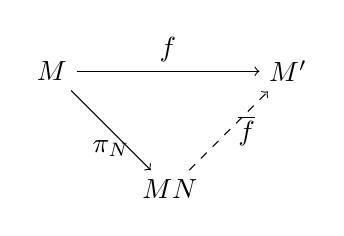
\begin{tikzpicture}
		\node (M) at (0,0) {$M$};
		\node (MS) at (3,0) {$M'$};
		\node (Q) at (1.5,-1.5) {\qraum{$M$}{$N$}};
		\draw[->, above] (M) to node {$f$} (MS);
		\draw[->, below] (M)  to node {$\pi_N$} (Q);
		\draw[->, right, dashed] (Q)  to node {$\overline{f}$} (MS);
		\end{tikzpicture}
	\end{center}
\end{proposition}
\begin{proof}
	Analog zu LAAG 1 III.7.9. Man zeigt, dass jedes $\overline{f}\in\Hom_K(\qraum{M}{N},M')$
	\begin{align}
		\overline{f}(x+N)=f(x)\quad (x\in M)\notag
	\end{align}
	erfüllen muss, und dass dies wiederum eine wohldefinierte Abbildung liefert. %TODO: Verlinkung
\end{proof}

\begin{lemma}
	Durch $U\mapsto \pi_N(U)$ wird eine Bijektion gegeben zwischen
	\begin{itemize}
		\item den Untermoduln von $M$, die $N$ enthalten
		\item den Untermoduln von $\qraum{M}{N}$.
	\end{itemize}
\end{lemma}
\begin{proof}
	Sei $\mathcal{U}$ die Menge der Untermoduln von $M$, die $N$ enthalten, $\overline{\mathcal{U}}$ die Menge der Untermoduln von $\qraum{M}{N}$.
	\begin{itemize}
		\item $U\in\mathcal{U}\Rightarrow \pi_N(U)\in\overline{\mathcal{U}}$: klar, da $\pi_N$ ein Homomorphismus ist
		\item $\overline{U}\in\overline{\mathcal{U}}\Rightarrow \pi_N^{-1}\in\mathcal{U}$: klar, da $\pi_N$ ein Homomorphismus ist und $N=\Ker(\pi_N)=\pi_N^{-1}(\{0\})\subseteq \pi_N^{-1}(\overline{U})$
		\item $\overline{U}\in\overline{\mathcal{U}}\Rightarrow\pi_N(\pi_N^{-1}(\overline{U}))=\overline{U}$: klar, da $\pi_N$ surjektiv
		\item $U\in\mathcal{U}\Rightarrow \pi_N^{-1}(\pi_N(U))=U$:
		\begin{align}
			\pi_N^{-1}(\pi_N(U)) &= \bigcup_{x\in U} \pi_N^{-1}(\pi_N(x)) \notag \\
			&= \bigcup_{x\in U} \pi_N^{-1}(x+N) \notag \\
			&= \bigcup_{x\in U}(x+N) \notag \\
			&= U+N=U\notag
		\end{align}
	\end{itemize}
\end{proof}
\section{Der Elementarteilersatz}

Sei $R$ Hauptidealring.

\begin{definition}
	Seien $a,b,x,y\in R$. Für $i,j\in\{1,...,n\}$ ist
	\begin{align}
		E_{ij} = (\delta_{\sigma,i},...,\delta_{\mu,j})_{\sigma,\mu}\in\Mat_n(\real)\notag
	\end{align}
	Sei
	\begin{align}
		E_{ij}(a,b,x,y) = \mathbbm{1}_n-E_{ii}-E_{jj}+aE_{ii}+bE_{ij}+xE_{jj}+yE_{ji}\notag
	\end{align}
	%TODO: Matrix ergänzen von Pascal
\end{definition}

\begin{lemma}
	Ist $ax-by\in R^\times$, so ist
	\begin{align}
		E_{ij}(a,b,x,y)\in \GL_n(\real)\notag
	\end{align}
\end{lemma}
\begin{proof}
	Folgt aus LAAG1 IV.3.4, da
	%TODO: Verlinkung
	\begin{align}
		\det(E_{ij}(a,b,x,y))=ax-by\in R^\times\notag
	\end{align}
	Oder direkt: Das Inverse ist $E_{ij}(xc^{-1},bc^{-1}, ac^{-1},-yc^{-1})$, zum Beispiel
	\begin{align}
		\begin{pmatrix} a & b \\ y & x\end{pmatrix}\begin{pmatrix}xc^{-1} & -bc^{-1} \\ -yc^{-1} & ac^{-1}\end{pmatrix}=\begin{pmatrix}(ax-by)c^{-1} & 0 \\ 0 & (ax-by)c^{-1}\end{pmatrix}\notag
	\end{align}
\end{proof}

\begin{remark}
	Multiplikation mit $E_{ij}(a,b,x,y)$ von links an $(a_1,...,a_n)^t\in\Mat_n(\real)$
	%TODO: konnte den Rest nicht erkennen, noch ergänzen
\end{remark}

\begin{theorem}[Elementarteilersatz für Matrizen]
	Sei $A\in\Mat_{m\times n}(\real)$. Es gibt
	\begin{align}
		0\le r \le\min\{n,m\}\notag \\
		S\in\GL_m(\real)\notag \\
		T\in\GL_n(\real)\notag
	\end{align}
	mit 
	\begin{align}
		SAT &= \diag(d_1,...,d_r,Q) \notag \\
		0&=Q\in\Mat_{m-r\times n-r}\notag
	\end{align}
	wobei $d_i\in R\backslash\{0\}$ mit $d_i\mid d_{i+1}$ für $i=1,...,n-1$
\end{theorem}
\section{Zyklische Vektorräume}

Sei $K$ ein Körper, $V$ ein $n$-dimensionaler $K$-Vektorraum, $f\in\End_K(V)$.

\begin{remark}
	Wir betrachten $V$ als $K[t]$-Modul mit $P(t)\cdot x=P(f)(x)$, vergleiche \proplbl{8_1_2}. \\
	\emph{Erinnerung:} $V$ heißt $f$-zyklisch $\iff \exists x\in V$ mit $V=\Span_K(x,f(x),f^2(x),...)$. Ist $k$ minimal mit $f^k(x)\in\Span_K(x,f(x),f^2(x),...,f^{k-1}(x))$, so ist $\underbrace{(x,...,f^{k-1}(x))}_{B}$ eine Basis von $V$ und $M_B(f)=M_{\chi_f}$.
\end{remark}

\begin{proposition}
	\proplbl{8_7_2}
	Es gibt einen $K[t]$-Modul-Isomorphismus
	\begin{align}
		V\cong \bigoplus_{i=1}^m\qraum{K[t]}{(P_i)}\notag
	\end{align}
	mit normierten Polynomen $P_1,...,P_m\in K[t]$, die $P_i\mid P_{i+1}$ $\forall i$ erfüllen.
\end{proposition}
\begin{proof}
	Nach \propref{8_6_13} ($K[t]$ Hauptidealring) ist 
	\begin{align}
		V\cong K[t]^r\oplus\bigoplus_{i=1}^m \qraum{K[t]}{K[t]\cdot P_i}\notag
	\end{align}
	mit $P_i\in K[t]\backslash K$, $P_i\mid P_{i+1}$ $\forall i$. Da $\dim_K(K[t])=\infty>\dim_K(V)$ ist, ist $r=0$, und wir können ohne Einschränkung $P_i$ normiert annehmen.
\end{proof}

\begin{lemma}
	Für $P\in K[t]$ sei $W:=\qraum{K[t]}{(P)}$. Durch $f_t(x)=\overline{t}x$ wird $f_t\in\End_K(W)$ definiert, wobei $\overline{t}=t+(P)=\pi_{(P)}(t)\in \qraum{K[t]}{(P)}$. Genau dann ist $\phi\in\Hom_K(V,W)$ ein $K[t]$-Modul-Homomorphismus, wenn $\phi(f(x))=f_t(\phi(x))$ $\forall x\in V$.
\end{lemma}
\begin{proof}
	\begin{itemize}
		\item $f_t\in\End_K(W)$: klar
		\item Es gilt
		\begin{align}
			\phi\text{ ist } K[t]\text{-Modul-Homomorphismus} &\iff \phi(ax)=a\phi(x)\quad\forall a\in K[t],\forall x\in V \notag \\
			&\iff \phi(tx)=t\phi(x)\quad\forall x\in V \notag \\
			&\iff \phi(f(x))=f_t(\phi(x))\quad\forall x\in V\notag
		\end{align}
	\end{itemize}
\end{proof}

\begin{proposition}
	Genau dann ist $\qraum{K[t]}{(P)}$ (als $K[t]$-Modul), wenn $V$ $f$-zyklisch ist. In diesem Fall ist
	\begin{align}
		\chi_f=P_f=P\notag
	\end{align}
\end{proposition}
\begin{proof}
	\begin{itemize}
		\item Hinrichtung: Der $K$-Vektorraum $W=\qraum{K[t]}{(P)}$ ist erzeugt von $1,\overline{t}=f_t(1),\overline{t}^2=f^2_t(1),...$, wobei $\overline{t}=t+(P)$ und somit ist $W$ $f_t$-zyklisch mit Basis $C=(1,\overline{t},\overline{t}^2,...,\overline{t}^{n-1})$, wobei $n=\deg(P)$. Auch ist $M_C(f_t)=M_P$. Ist $V\cong\qraum{K[t]}{(P)}$ so ist dann $V$ $f$-zyklisch.
		\item Rückrichtung: Ist umgekehrt $V$ ein $K$-Vektorraum mit Basis $B=(x,f(x),...,f^{n-1}(x))$, so ist $M_B(f)=M_P$ für $P=\chi_f$. Der $K$-Vektorraum-Homomorphismus $\phi:V\to W=\qraum{K[t]}{(P)}$ gegeben durch $\phi(f^i(x))=t^i$ ist dann ein $K[t]$-Modul-Isomorphismus.
		\item Ist $V\cong W$ als $K[t]$-Modul, so ist $\chi_f=\chi_{f_t}$, $P_f=P_{f_t}$. Aus $M_C(f_t)=M_P$ folgt somit 
		\begin{align}
			\chi_f=\chi_{f_t}=P\notag
		\end{align}
		Ist $0\neq Q\in K[t]$ mit $\deg(Q)<\deg(P)$, so ist
		\begin{align}
			Q(f_t)(1)=Q(\overline{t})\neq 0\notag
		\end{align}
		da $Q\neq 0$ und $C$ Basis, insbesondere $Q(f_t)\neq 0\in\End_K(\qraum{K[t]}{(P)})$. Da $P_{f_t}\mid \chi_{f_t}$ gilt, folgt 
		\begin{align}
			P_f=P_{f_t}=\chi_{f_t}=P\notag
		\end{align}
	\end{itemize}
\end{proof}

\begin{conclusion}
	$V$ ist direkte Summe $f$-zyklischer Untervektorräume.
\end{conclusion}

\begin{conclusion}
	Es gilt
	\begin{align}
		\chi_f\mid (P_f)^n\notag
	\end{align}
	Insbesondere haben $\chi_f$ und $P_f$ die selben irreduziblen Faktoren.
\end{conclusion}
\begin{proof}
	In der Situation von \propref{8_7_2} ist
	\begin{align}
		\chi_f &= \prod_{i=1}^m P_i\notag \\
		P_f &= \kgV(P_1,...,P_m)=P_m\notag
	\end{align}
	Da $P_i\mid P_m$ für alle $i$ folgt $\chi_f\mid (P_m)^m$, insbesondere $\chi_f\mid (P_m)^n$, denn $m\le n$.
\end{proof}

\begin{conclusion}[\person{Frobenius}-Normalform]
	Es gibt eine Basis $B$ von $V$, für die 
	\begin{align}
		M_B(f)=\diag(M_{P_1},...,M_{P_m})\notag
	\end{align}
	mit $P_1,...,P_m\in K[t]$ normiert, die $P_i\mid P_{i+1}$ erfüllen.
\end{conclusion}

\begin{remark}
	Im Gegensatz zur \person{Jordan}-Normalform existiert die \person{Frobenius}-Normalform für beliebige Körper $K$ und beliebige Endomorphismen $f$. Man kann zeigen, dass die \person{Frobenius}-Normalform eines Endomorphismus $f$ eindeutig bestimmt ist.
\end{remark}

\part*{Anhang}
\addcontentsline{toc}{part}{Anhang}
\appendix

\chapter{Listen}
\section{Liste der Theoreme}
\theoremlisttype{allname}
\listtheorems{theorem}

\pagebreak
\section{Liste der benannten Sätze, Lemmata und Folgerungen}
\theoremlisttype{optname}
\listtheorems{proposition,lemma,conclusion}

\pagebreak
\section{Liste der Mathematica/WolframAlpha-Befehle}
\smiley{} für faule Mathematiker \smiley{} \\
\theoremlisttype{allname}
\listtheorems{mathematica}

%\printglossary[type=\acronymtype]

\printindex

\end{document}